% Options for packages loaded elsewhere
\PassOptionsToPackage{unicode}{hyperref}
\PassOptionsToPackage{hyphens}{url}
%
\documentclass[
]{article}
\usepackage{amsmath,amssymb}
\usepackage{iftex}
\ifPDFTeX
  \usepackage[T1]{fontenc}
  \usepackage[utf8]{inputenc}
  \usepackage{textcomp} % provide euro and other symbols
\else % if luatex or xetex
  \usepackage{unicode-math} % this also loads fontspec
  \defaultfontfeatures{Scale=MatchLowercase}
  \defaultfontfeatures[\rmfamily]{Ligatures=TeX,Scale=1}
\fi
\usepackage{lmodern}
\ifPDFTeX\else
  % xetex/luatex font selection
\fi
% Use upquote if available, for straight quotes in verbatim environments
\IfFileExists{upquote.sty}{\usepackage{upquote}}{}
\IfFileExists{microtype.sty}{% use microtype if available
  \usepackage[]{microtype}
  \UseMicrotypeSet[protrusion]{basicmath} % disable protrusion for tt fonts
}{}
\makeatletter
\@ifundefined{KOMAClassName}{% if non-KOMA class
  \IfFileExists{parskip.sty}{%
    \usepackage{parskip}
  }{% else
    \setlength{\parindent}{0pt}
    \setlength{\parskip}{6pt plus 2pt minus 1pt}}
}{% if KOMA class
  \KOMAoptions{parskip=half}}
\makeatother
\usepackage{xcolor}
\usepackage[margin=1in]{geometry}
\usepackage{color}
\usepackage{fancyvrb}
\newcommand{\VerbBar}{|}
\newcommand{\VERB}{\Verb[commandchars=\\\{\}]}
\DefineVerbatimEnvironment{Highlighting}{Verbatim}{commandchars=\\\{\}}
% Add ',fontsize=\small' for more characters per line
\usepackage{framed}
\definecolor{shadecolor}{RGB}{248,248,248}
\newenvironment{Shaded}{\begin{snugshade}}{\end{snugshade}}
\newcommand{\AlertTok}[1]{\textcolor[rgb]{0.94,0.16,0.16}{#1}}
\newcommand{\AnnotationTok}[1]{\textcolor[rgb]{0.56,0.35,0.01}{\textbf{\textit{#1}}}}
\newcommand{\AttributeTok}[1]{\textcolor[rgb]{0.13,0.29,0.53}{#1}}
\newcommand{\BaseNTok}[1]{\textcolor[rgb]{0.00,0.00,0.81}{#1}}
\newcommand{\BuiltInTok}[1]{#1}
\newcommand{\CharTok}[1]{\textcolor[rgb]{0.31,0.60,0.02}{#1}}
\newcommand{\CommentTok}[1]{\textcolor[rgb]{0.56,0.35,0.01}{\textit{#1}}}
\newcommand{\CommentVarTok}[1]{\textcolor[rgb]{0.56,0.35,0.01}{\textbf{\textit{#1}}}}
\newcommand{\ConstantTok}[1]{\textcolor[rgb]{0.56,0.35,0.01}{#1}}
\newcommand{\ControlFlowTok}[1]{\textcolor[rgb]{0.13,0.29,0.53}{\textbf{#1}}}
\newcommand{\DataTypeTok}[1]{\textcolor[rgb]{0.13,0.29,0.53}{#1}}
\newcommand{\DecValTok}[1]{\textcolor[rgb]{0.00,0.00,0.81}{#1}}
\newcommand{\DocumentationTok}[1]{\textcolor[rgb]{0.56,0.35,0.01}{\textbf{\textit{#1}}}}
\newcommand{\ErrorTok}[1]{\textcolor[rgb]{0.64,0.00,0.00}{\textbf{#1}}}
\newcommand{\ExtensionTok}[1]{#1}
\newcommand{\FloatTok}[1]{\textcolor[rgb]{0.00,0.00,0.81}{#1}}
\newcommand{\FunctionTok}[1]{\textcolor[rgb]{0.13,0.29,0.53}{\textbf{#1}}}
\newcommand{\ImportTok}[1]{#1}
\newcommand{\InformationTok}[1]{\textcolor[rgb]{0.56,0.35,0.01}{\textbf{\textit{#1}}}}
\newcommand{\KeywordTok}[1]{\textcolor[rgb]{0.13,0.29,0.53}{\textbf{#1}}}
\newcommand{\NormalTok}[1]{#1}
\newcommand{\OperatorTok}[1]{\textcolor[rgb]{0.81,0.36,0.00}{\textbf{#1}}}
\newcommand{\OtherTok}[1]{\textcolor[rgb]{0.56,0.35,0.01}{#1}}
\newcommand{\PreprocessorTok}[1]{\textcolor[rgb]{0.56,0.35,0.01}{\textit{#1}}}
\newcommand{\RegionMarkerTok}[1]{#1}
\newcommand{\SpecialCharTok}[1]{\textcolor[rgb]{0.81,0.36,0.00}{\textbf{#1}}}
\newcommand{\SpecialStringTok}[1]{\textcolor[rgb]{0.31,0.60,0.02}{#1}}
\newcommand{\StringTok}[1]{\textcolor[rgb]{0.31,0.60,0.02}{#1}}
\newcommand{\VariableTok}[1]{\textcolor[rgb]{0.00,0.00,0.00}{#1}}
\newcommand{\VerbatimStringTok}[1]{\textcolor[rgb]{0.31,0.60,0.02}{#1}}
\newcommand{\WarningTok}[1]{\textcolor[rgb]{0.56,0.35,0.01}{\textbf{\textit{#1}}}}
\usepackage{graphicx}
\makeatletter
\def\maxwidth{\ifdim\Gin@nat@width>\linewidth\linewidth\else\Gin@nat@width\fi}
\def\maxheight{\ifdim\Gin@nat@height>\textheight\textheight\else\Gin@nat@height\fi}
\makeatother
% Scale images if necessary, so that they will not overflow the page
% margins by default, and it is still possible to overwrite the defaults
% using explicit options in \includegraphics[width, height, ...]{}
\setkeys{Gin}{width=\maxwidth,height=\maxheight,keepaspectratio}
% Set default figure placement to htbp
\makeatletter
\def\fps@figure{htbp}
\makeatother
\setlength{\emergencystretch}{3em} % prevent overfull lines
\providecommand{\tightlist}{%
  \setlength{\itemsep}{0pt}\setlength{\parskip}{0pt}}
\setcounter{secnumdepth}{-\maxdimen} % remove section numbering
\ifLuaTeX
  \usepackage{selnolig}  % disable illegal ligatures
\fi
\IfFileExists{bookmark.sty}{\usepackage{bookmark}}{\usepackage{hyperref}}
\IfFileExists{xurl.sty}{\usepackage{xurl}}{} % add URL line breaks if available
\urlstyle{same}
\hypersetup{
  pdftitle={Exploratory Data Analysis},
  pdfauthor={Giovanni Saraceno},
  hidelinks,
  pdfcreator={LaTeX via pandoc}}

\title{Exploratory Data Analysis}
\author{Giovanni Saraceno}
\date{}

\begin{document}
\maketitle

{
\setcounter{tocdepth}{2}
\tableofcontents
}
Differently from \textbf{inferential statistics} (it will be addressed
in the following sections) that deals with uncertainties in estimates
and inferences about one or more populations, \textbf{Exploratory Data
Analysis} aims to reveal interesting patterns and help to prepare the
data in the best way for the following analyses.\\
It can be roughly summarized in three big parts:

\begin{enumerate}
\def\labelenumi{\arabic{enumi}.}
\tightlist
\item
  \emph{Structure and summary of data}: To check the type of variables
  in the data set and compute location indexes (e.g., mean, median),
  variability indexes (e.g., variance) of the variables of interest
\item
  \emph{Exploratory plots}: Histograms, box plots, bar plots,
  correlogram or scatter plots (e.g., skeweness, outliers)
\item
  \emph{Preprocessing step}: Are there any NAs? Missing values? Integer
  variables to be converted in factors?
\end{enumerate}

We will show the code using classical functions in R base and more
recent \texttt{tidyverse} and \texttt{ggplot2}.

\begin{Shaded}
\begin{Highlighting}[]
\FunctionTok{library}\NormalTok{(tidyverse)}
\end{Highlighting}
\end{Shaded}

\begin{verbatim}
## Warning: il pacchetto 'tidyverse' è stato creato con R versione 4.3.2
\end{verbatim}

\begin{verbatim}
## Warning: il pacchetto 'ggplot2' è stato creato con R versione 4.3.3
\end{verbatim}

\begin{verbatim}
## Warning: il pacchetto 'stringr' è stato creato con R versione 4.3.3
\end{verbatim}

\begin{verbatim}
## Warning: il pacchetto 'lubridate' è stato creato con R versione 4.3.2
\end{verbatim}

\begin{verbatim}
## -- Attaching core tidyverse packages ------------------------ tidyverse 2.0.0 --
## v dplyr     1.1.3     v readr     2.1.4
## v forcats   1.0.0     v stringr   1.5.1
## v ggplot2   3.5.1     v tibble    3.2.1
## v lubridate 1.9.3     v tidyr     1.3.0
## v purrr     1.0.2     
## -- Conflicts ------------------------------------------ tidyverse_conflicts() --
## x dplyr::filter() masks stats::filter()
## x dplyr::lag()    masks stats::lag()
## i Use the conflicted package (<http://conflicted.r-lib.org/>) to force all conflicts to become errors
\end{verbatim}

\begin{Shaded}
\begin{Highlighting}[]
\FunctionTok{library}\NormalTok{(dplyr)}
\end{Highlighting}
\end{Shaded}

We consider the data set \texttt{peso.Rdata} defined in the Introduction
notes.

\begin{Shaded}
\begin{Highlighting}[]
\NormalTok{dati }\OtherTok{\textless{}{-}} \FunctionTok{read.table}\NormalTok{(}\StringTok{"../Introduction/peso.txt"}\NormalTok{, }\AttributeTok{sep=}\StringTok{";"}\NormalTok{) }
\end{Highlighting}
\end{Shaded}

\begin{Shaded}
\begin{Highlighting}[]
\FunctionTok{str}\NormalTok{(dati)}
\end{Highlighting}
\end{Shaded}

\begin{verbatim}
## 'data.frame':    50 obs. of  4 variables:
##  $ X: chr  "C" "V" "S" "C" ...
##  $ Y: chr  "S" "L" "A" "L" ...
##  $ Z: int  3 3 2 3 1 0 0 3 0 0 ...
##  $ W: num  67.4 92 69.6 62.2 62.8 ...
\end{verbatim}

\begin{Shaded}
\begin{Highlighting}[]
\FunctionTok{attach}\NormalTok{(dati)}
\end{Highlighting}
\end{Shaded}

Generally, a data set contains information about a random sample. For
each observation (rows), characteristics, also called variables (data
set columns), are recorded. This means that the data represent
realizations of one or more measurements performed on a sample of
individuals.

Variables can be classified as:

\emph{Qualitative (categorical)}: These express characteristics that
cannot be measured numerically but allow assigning a sample observation
to a category or group. For example, the variables X and Y are
categorical. If there is no intrinsic order, the variables are called
nominal, whereas if the values can be ordered, they are ordinal.
\emph{Quantitative (numerical)}: The measurements are expressed as
numbers. Numerical data can be continuous, like the variable W
representing weight, or discrete, like the variable Z, representing the
number of dependents.

\hypertarget{discrete-variables}{%
\subsection{Discrete Variables}\label{discrete-variables}}

Discrete variables can take on a finite number of values. Both
qualitative and discrete numerical variables fall into this category. In
these cases, it is useful to examine the frequency distribution of all
its values. In R, the \texttt{table()} function is used:

\begin{Shaded}
\begin{Highlighting}[]
\FunctionTok{table}\NormalTok{(X)}
\end{Highlighting}
\end{Shaded}

\begin{verbatim}
## X
##  C  N  S  V 
## 10 12 16 12
\end{verbatim}

\begin{Shaded}
\begin{Highlighting}[]
\FunctionTok{table}\NormalTok{(Y)}
\end{Highlighting}
\end{Shaded}

\begin{verbatim}
## Y
##  A  L  O  S 
## 13 12  9 16
\end{verbatim}

\begin{Shaded}
\begin{Highlighting}[]
\FunctionTok{table}\NormalTok{(Z)}
\end{Highlighting}
\end{Shaded}

\begin{verbatim}
## Z
##  0  1  2  3  4 
## 14  7  8 11 10
\end{verbatim}

The same result can be obtained with the \texttt{summary()} function:

\begin{Shaded}
\begin{Highlighting}[]
\FunctionTok{summary}\NormalTok{(X)}
\end{Highlighting}
\end{Shaded}

\begin{verbatim}
##    Length     Class      Mode 
##        50 character character
\end{verbatim}

Alternatively, we can calculate relative frequencies by dividing by the
total number of observations:

\begin{Shaded}
\begin{Highlighting}[]
\FunctionTok{table}\NormalTok{(X) }\SpecialCharTok{/} \FunctionTok{length}\NormalTok{(X)}
\end{Highlighting}
\end{Shaded}

\begin{verbatim}
## X
##    C    N    S    V 
## 0.20 0.24 0.32 0.24
\end{verbatim}

\begin{Shaded}
\begin{Highlighting}[]
\FunctionTok{table}\NormalTok{(Y) }\SpecialCharTok{/} \FunctionTok{length}\NormalTok{(Y)}
\end{Highlighting}
\end{Shaded}

\begin{verbatim}
## Y
##    A    L    O    S 
## 0.26 0.24 0.18 0.32
\end{verbatim}

\begin{Shaded}
\begin{Highlighting}[]
\FunctionTok{table}\NormalTok{(Z) }\SpecialCharTok{/} \FunctionTok{length}\NormalTok{(Z)}
\end{Highlighting}
\end{Shaded}

\begin{verbatim}
## Z
##    0    1    2    3    4 
## 0.28 0.14 0.16 0.22 0.20
\end{verbatim}

The frequency table can be represented using a bar plot:

\begin{Shaded}
\begin{Highlighting}[]
\FunctionTok{plot}\NormalTok{(}\FunctionTok{table}\NormalTok{(X) }\SpecialCharTok{/} \FunctionTok{length}\NormalTok{(X))}
\end{Highlighting}
\end{Shaded}

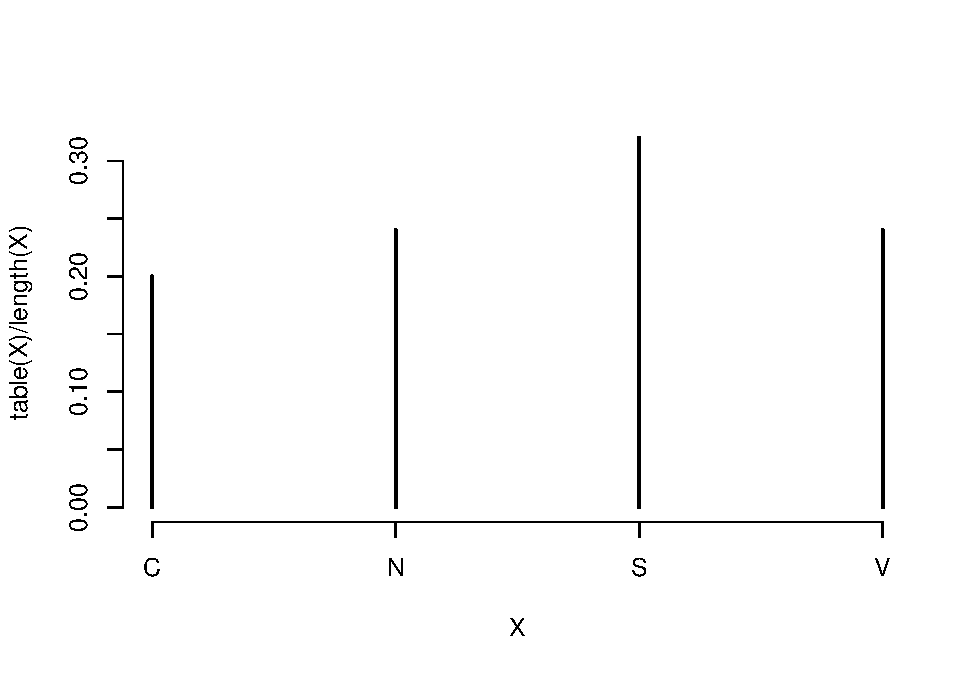
\includegraphics{EDA_files/figure-latex/unnamed-chunk-7-1.pdf}

If there is an intrinsic order, cumulative frequencies can be calculated
and visualized:

\begin{Shaded}
\begin{Highlighting}[]
\NormalTok{Y }\OtherTok{\textless{}{-}} \FunctionTok{ordered}\NormalTok{(Y, }\AttributeTok{levels =} \FunctionTok{c}\NormalTok{(}\StringTok{"A"}\NormalTok{, }\StringTok{"O"}\NormalTok{, }\StringTok{"S"}\NormalTok{, }\StringTok{"L"}\NormalTok{))}
\FunctionTok{cumsum}\NormalTok{(}\FunctionTok{table}\NormalTok{(Y) }\SpecialCharTok{/} \FunctionTok{length}\NormalTok{(Y))}
\end{Highlighting}
\end{Shaded}

\begin{verbatim}
##    A    O    S    L 
## 0.26 0.44 0.76 1.00
\end{verbatim}

\begin{Shaded}
\begin{Highlighting}[]
\FunctionTok{plot}\NormalTok{(}\FunctionTok{ecdf}\NormalTok{(Y))}
\end{Highlighting}
\end{Shaded}

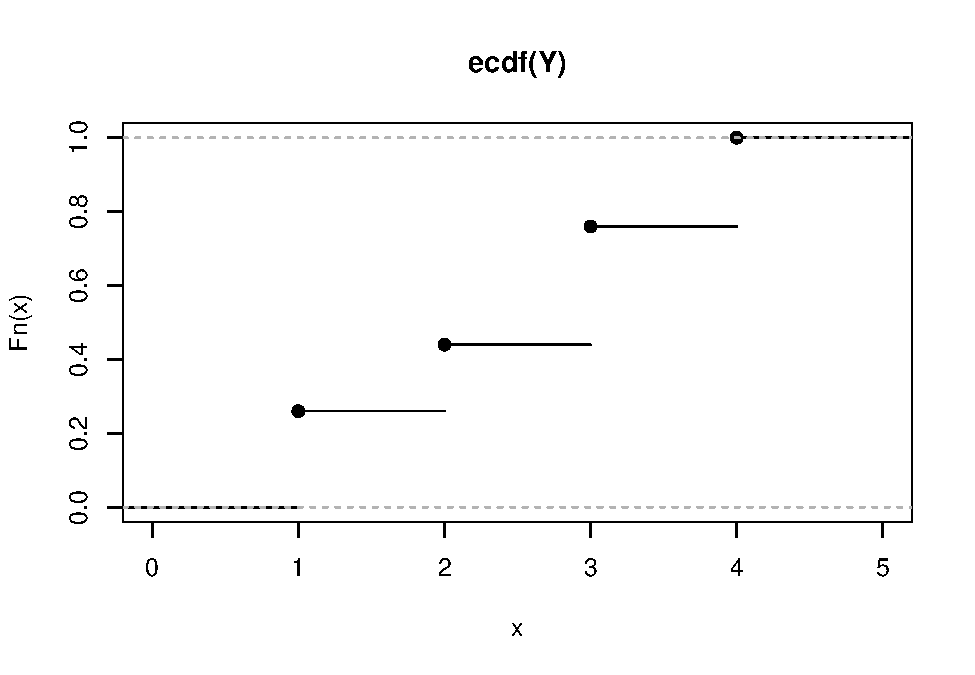
\includegraphics{EDA_files/figure-latex/unnamed-chunk-8-1.pdf}

For numerical variables:

\begin{Shaded}
\begin{Highlighting}[]
\FunctionTok{cumsum}\NormalTok{(}\FunctionTok{table}\NormalTok{(Z) }\SpecialCharTok{/} \FunctionTok{length}\NormalTok{(Z))}
\end{Highlighting}
\end{Shaded}

\begin{verbatim}
##    0    1    2    3    4 
## 0.28 0.42 0.58 0.80 1.00
\end{verbatim}

\begin{Shaded}
\begin{Highlighting}[]
\FunctionTok{plot}\NormalTok{(}\FunctionTok{ecdf}\NormalTok{(Z))}
\end{Highlighting}
\end{Shaded}

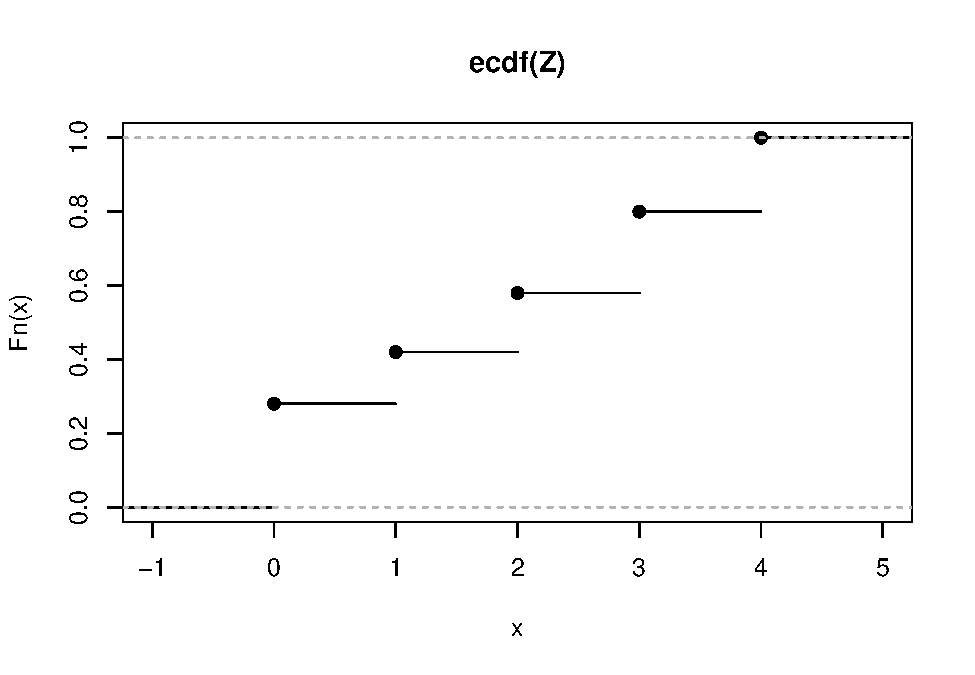
\includegraphics{EDA_files/figure-latex/unnamed-chunk-9-1.pdf}

If we try the same approach for the continuous variable W:

\begin{Shaded}
\begin{Highlighting}[]
\FunctionTok{table}\NormalTok{(W)}
\end{Highlighting}
\end{Shaded}

\begin{verbatim}
## W
## 33.8775213811631  35.415381519041 35.6541383784125 46.8793378145431 
##                1                1                1                1 
## 52.7563552228405 53.5093799191515 54.6999662397492 55.6815339944367 
##                1                1                1                1 
## 56.8334866492771 58.2672500739823 58.3348777630801 58.3741853493409 
##                1                1                1                1 
##  60.620274255931 62.1671633352717 62.4897250497831 62.8292713451724 
##                1                1                1                1 
## 65.3465638930294 65.4002856629698 66.2775496879411 67.3636262541611 
##                1                1                1                1 
## 67.6755853135583 68.4544098140893  68.740736621617 68.7978424311212 
##                1                1                1                1 
## 69.2732924143287 69.5525561112997 70.5068119580714 70.5337080538567 
##                1                1                1                1 
## 70.6596373620813 70.9898462988698 71.9264050204625 72.3093811329276 
##                1                1                1                1 
## 72.5118550761639 72.5875217892273 73.7989398733261 74.0285707226046 
##                1                1                1                1 
## 74.3343427103841 75.1902425061576 75.5592639184782 75.7420006340731 
##                1                1                1                1 
## 75.9049996280411 77.9022338200939 78.0231473179288 79.6829638948667 
##                1                1                1                1 
## 81.4791220807459 81.7437461127363 82.6824333573602 91.9674895901944 
##                1                1                1                1 
## 94.2333713818525 95.9258755494911 
##                1                1
\end{verbatim}

It provides no useful information because all values are different,
reflecting that W is described by a continuous random variable.

\hypertarget{continuous-variables}{%
\subsection{Continuous Variables}\label{continuous-variables}}

Let's now explore descriptive statistics for continuous numerical
variables.

Consider the following example: in a factory assembling devices, three
different production line organizations are tested over three days: the
current organization, old, and two new ones, new1 and new2. The
productivity, measured as the number of completed operations, is
recorded for 288 workers and stored in the data set organization.

\begin{Shaded}
\begin{Highlighting}[]
\NormalTok{organization }\OtherTok{\textless{}{-}} \FunctionTok{read.table}\NormalTok{(}\StringTok{"organizzazione.txt"}\NormalTok{, }\AttributeTok{sep=}\StringTok{","}\NormalTok{)}
\end{Highlighting}
\end{Shaded}

\begin{Shaded}
\begin{Highlighting}[]
\FunctionTok{str}\NormalTok{(organization)}
\end{Highlighting}
\end{Shaded}

\begin{verbatim}
## 'data.frame':    288 obs. of  3 variables:
##  $ old : int  676 676 680 681 682 681 686 685 689 686 ...
##  $ new1: int  732 732 734 733 736 738 738 736 737 736 ...
##  $ new2: int  731 731 730 732 733 733 734 730 732 733 ...
\end{verbatim}

\begin{Shaded}
\begin{Highlighting}[]
\FunctionTok{attach}\NormalTok{(organization)}
\end{Highlighting}
\end{Shaded}

Start by studying the variable old. Basic statistics include mean,
standard deviation, variance, median, minimum, and maximum:

\begin{Shaded}
\begin{Highlighting}[]
\FunctionTok{mean}\NormalTok{(old)}
\end{Highlighting}
\end{Shaded}

\begin{verbatim}
## [1] 705.3333
\end{verbatim}

\begin{Shaded}
\begin{Highlighting}[]
\FunctionTok{sd}\NormalTok{(old)}
\end{Highlighting}
\end{Shaded}

\begin{verbatim}
## [1] 10.2512
\end{verbatim}

\begin{Shaded}
\begin{Highlighting}[]
\FunctionTok{var}\NormalTok{(old)}
\end{Highlighting}
\end{Shaded}

\begin{verbatim}
## [1] 105.0871
\end{verbatim}

\begin{Shaded}
\begin{Highlighting}[]
\FunctionTok{median}\NormalTok{(old)}
\end{Highlighting}
\end{Shaded}

\begin{verbatim}
## [1] 706
\end{verbatim}

\begin{Shaded}
\begin{Highlighting}[]
\FunctionTok{range}\NormalTok{(old)}
\end{Highlighting}
\end{Shaded}

\begin{verbatim}
## [1] 676 729
\end{verbatim}

Empirical quantiles can be obtained with the \texttt{quantile()}
function:

\begin{Shaded}
\begin{Highlighting}[]
\FunctionTok{quantile}\NormalTok{(old)}
\end{Highlighting}
\end{Shaded}

\begin{verbatim}
##   0%  25%  50%  75% 100% 
##  676  699  706  713  729
\end{verbatim}

\begin{Shaded}
\begin{Highlighting}[]
\FunctionTok{quantile}\NormalTok{(old, }\FunctionTok{seq}\NormalTok{(}\DecValTok{0}\NormalTok{, }\DecValTok{1}\NormalTok{, }\FloatTok{0.1}\NormalTok{))  }\CommentTok{\# Deciles}
\end{Highlighting}
\end{Shaded}

\begin{verbatim}
##    0%   10%   20%   30%   40%   50%   60%   70%   80%   90%  100% 
## 676.0 692.0 697.0 700.0 703.0 706.0 708.0 711.0 714.0 718.3 729.0
\end{verbatim}

A summary of these key statistics can be obtained using the
\texttt{summary()} function:

\begin{Shaded}
\begin{Highlighting}[]
\FunctionTok{summary}\NormalTok{(old)}
\end{Highlighting}
\end{Shaded}

\begin{verbatim}
##    Min. 1st Qu.  Median    Mean 3rd Qu.    Max. 
##   676.0   699.0   706.0   705.3   713.0   729.0
\end{verbatim}

\begin{Shaded}
\begin{Highlighting}[]
\FunctionTok{summary}\NormalTok{(organization)}
\end{Highlighting}
\end{Shaded}

\begin{verbatim}
##       old             new1            new2      
##  Min.   :676.0   Min.   :671.0   Min.   :679.0  
##  1st Qu.:699.0   1st Qu.:688.0   1st Qu.:707.0  
##  Median :706.0   Median :699.0   Median :719.0  
##  Mean   :705.3   Mean   :700.8   Mean   :719.2  
##  3rd Qu.:713.0   3rd Qu.:711.2   3rd Qu.:730.2  
##  Max.   :729.0   Max.   :759.0   Max.   :758.0
\end{verbatim}

Frequency distributions of continuous numerical variables can be
visualized with histograms:

\begin{Shaded}
\begin{Highlighting}[]
\FunctionTok{hist}\NormalTok{(old)}
\end{Highlighting}
\end{Shaded}

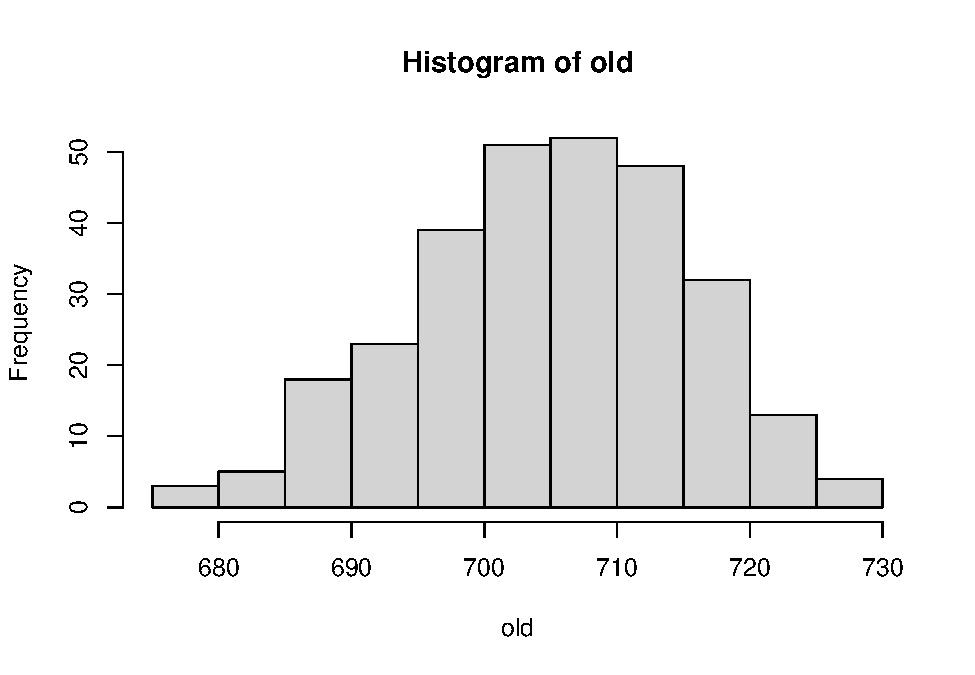
\includegraphics{EDA_files/figure-latex/unnamed-chunk-16-1.pdf}

\begin{Shaded}
\begin{Highlighting}[]
\FunctionTok{hist}\NormalTok{(old, }\AttributeTok{freq =} \ConstantTok{FALSE}\NormalTok{)  }\CommentTok{\# Density}
\end{Highlighting}
\end{Shaded}

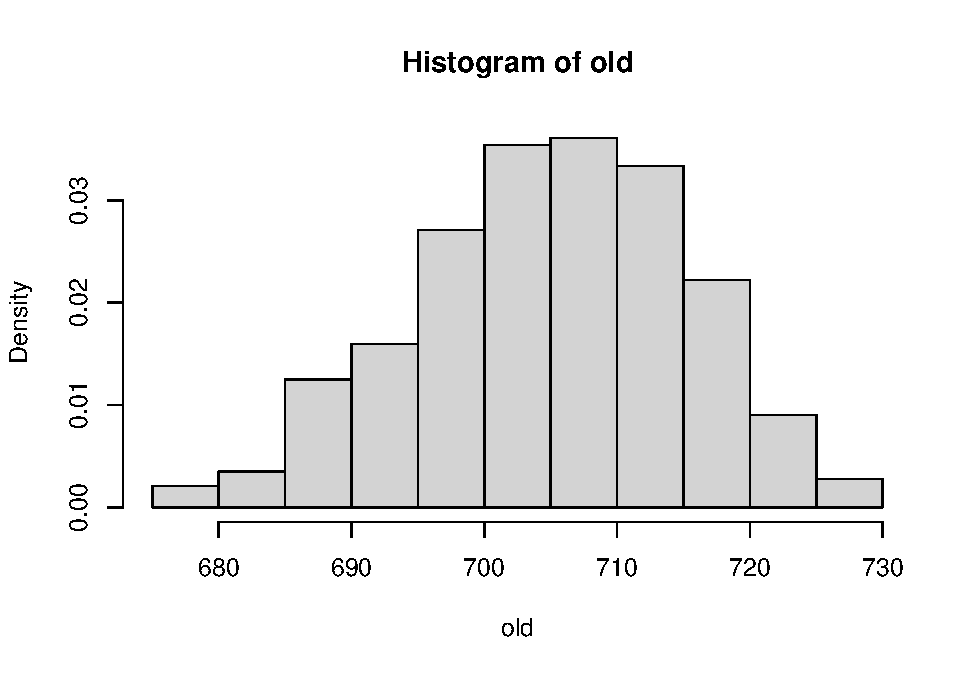
\includegraphics{EDA_files/figure-latex/unnamed-chunk-16-2.pdf}

\begin{Shaded}
\begin{Highlighting}[]
\FunctionTok{hist}\NormalTok{(old, }\AttributeTok{freq =} \ConstantTok{FALSE}\NormalTok{, }\AttributeTok{breaks =} \DecValTok{20}\NormalTok{)  }\CommentTok{\# Custom intervals}
\end{Highlighting}
\end{Shaded}

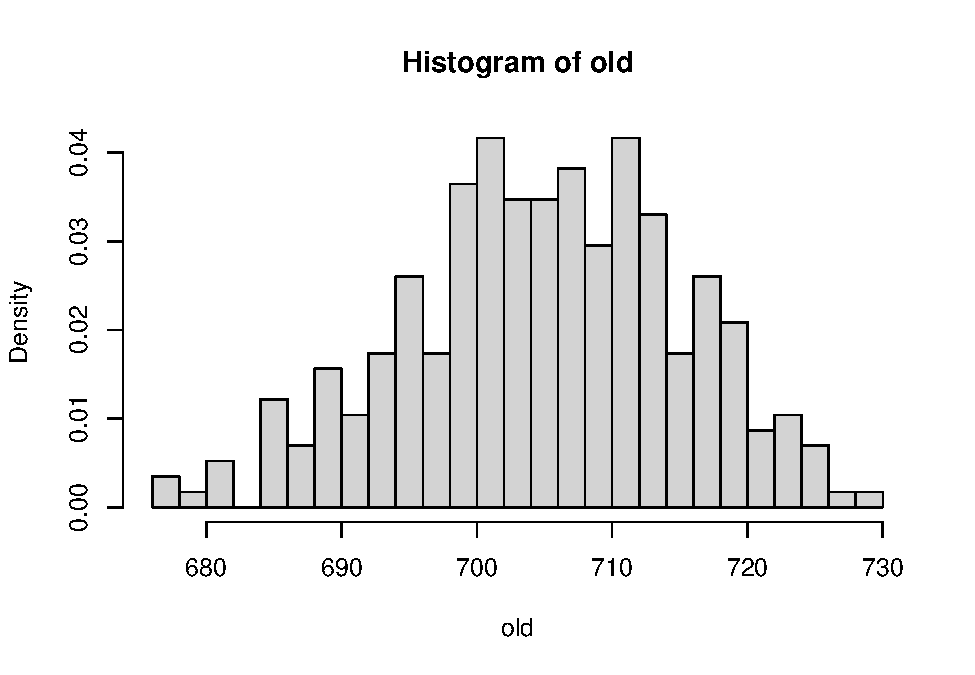
\includegraphics{EDA_files/figure-latex/unnamed-chunk-16-3.pdf}

The Freedman-Diaconis method for choosing interval widths:

\begin{Shaded}
\begin{Highlighting}[]
\FunctionTok{hist}\NormalTok{(old, }\AttributeTok{freq =} \ConstantTok{FALSE}\NormalTok{, }\AttributeTok{breaks =} \StringTok{"FD"}\NormalTok{)}
\end{Highlighting}
\end{Shaded}

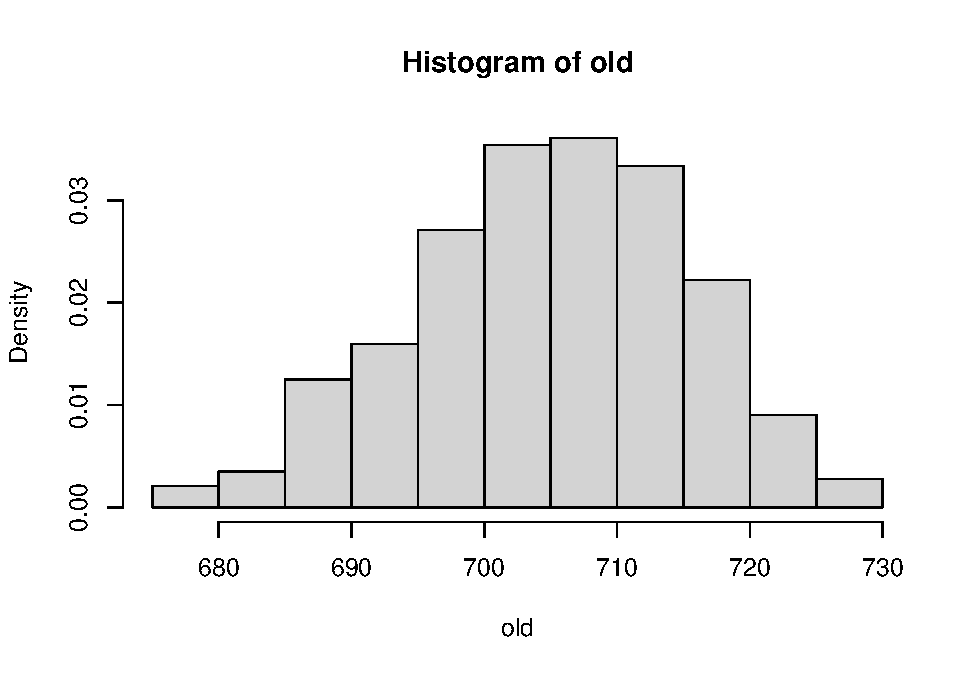
\includegraphics{EDA_files/figure-latex/unnamed-chunk-17-1.pdf}

Kernel density estimation provides a continuous approximation of the
empirical probability density:

\begin{Shaded}
\begin{Highlighting}[]
\FunctionTok{plot}\NormalTok{(}\FunctionTok{density}\NormalTok{(old))}
\end{Highlighting}
\end{Shaded}

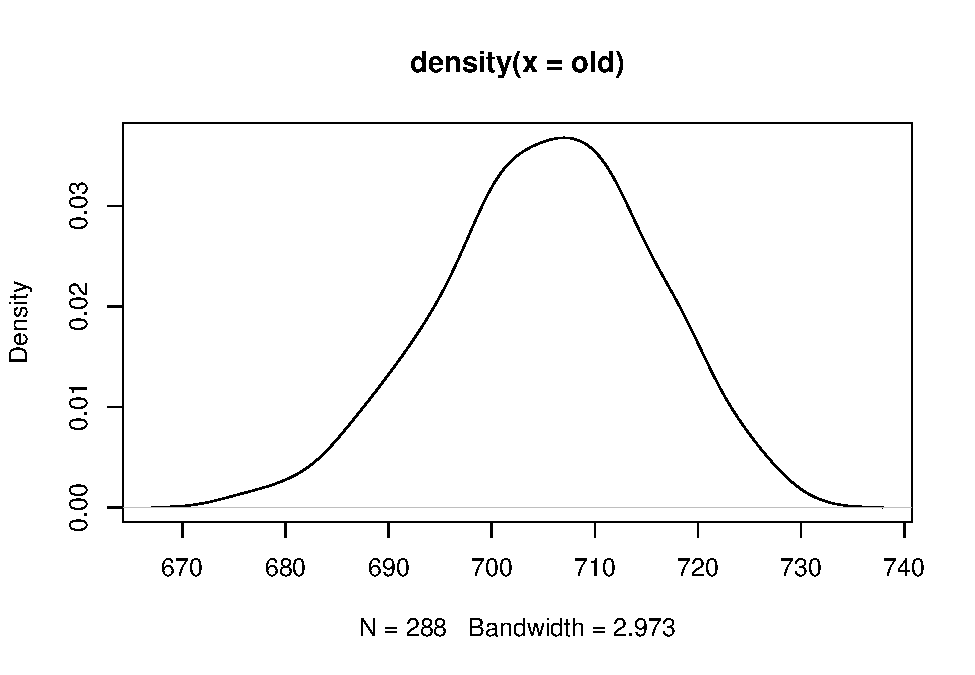
\includegraphics{EDA_files/figure-latex/unnamed-chunk-18-1.pdf}

To compare with a known probability density (e.g., normal distribution):

\begin{Shaded}
\begin{Highlighting}[]
\FunctionTok{hist}\NormalTok{(old, }\AttributeTok{freq =} \ConstantTok{FALSE}\NormalTok{, }\AttributeTok{breaks =} \FunctionTok{seq}\NormalTok{(}\DecValTok{665}\NormalTok{, }\DecValTok{740}\NormalTok{, }\DecValTok{5}\NormalTok{), }\AttributeTok{ylim =} \FunctionTok{c}\NormalTok{(}\DecValTok{0}\NormalTok{, }\FloatTok{0.04}\NormalTok{))}
\FunctionTok{curve}\NormalTok{(}\FunctionTok{dnorm}\NormalTok{(x, }\AttributeTok{mean =} \FunctionTok{mean}\NormalTok{(old), }\AttributeTok{sd =} \FunctionTok{sd}\NormalTok{(old)), }\AttributeTok{col =} \StringTok{"red"}\NormalTok{, }\AttributeTok{add =} \ConstantTok{TRUE}\NormalTok{)}
\end{Highlighting}
\end{Shaded}

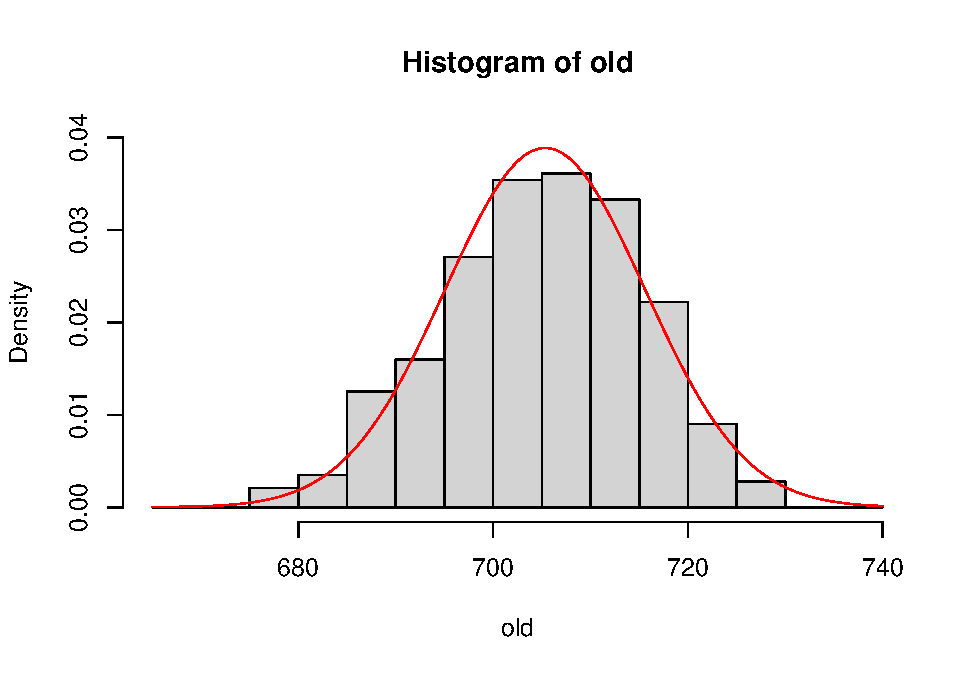
\includegraphics{EDA_files/figure-latex/unnamed-chunk-19-1.pdf}

The empirical cumulative distribution function (CDF):

\begin{Shaded}
\begin{Highlighting}[]
\FunctionTok{plot}\NormalTok{(}\FunctionTok{ecdf}\NormalTok{(old))}
\FunctionTok{curve}\NormalTok{(}\FunctionTok{pnorm}\NormalTok{(x, }\AttributeTok{mean =} \FunctionTok{mean}\NormalTok{(old), }\AttributeTok{sd =} \FunctionTok{sd}\NormalTok{(old)), }\AttributeTok{add =} \ConstantTok{TRUE}\NormalTok{, }\AttributeTok{col =} \StringTok{"red"}\NormalTok{)}
\end{Highlighting}
\end{Shaded}

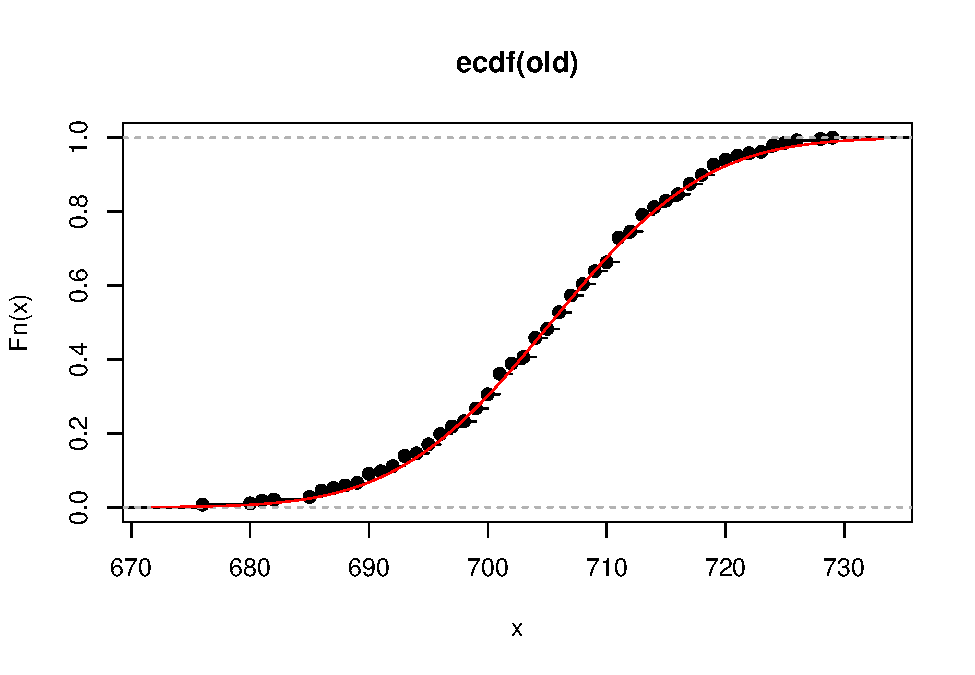
\includegraphics{EDA_files/figure-latex/unnamed-chunk-20-1.pdf}

A QQ-plot compares the data against theoretical quantiles of a normal
distribution:

\begin{Shaded}
\begin{Highlighting}[]
\FunctionTok{qqnorm}\NormalTok{(old)}
\FunctionTok{qqline}\NormalTok{(old, }\AttributeTok{col =} \StringTok{"red"}\NormalTok{)}
\end{Highlighting}
\end{Shaded}

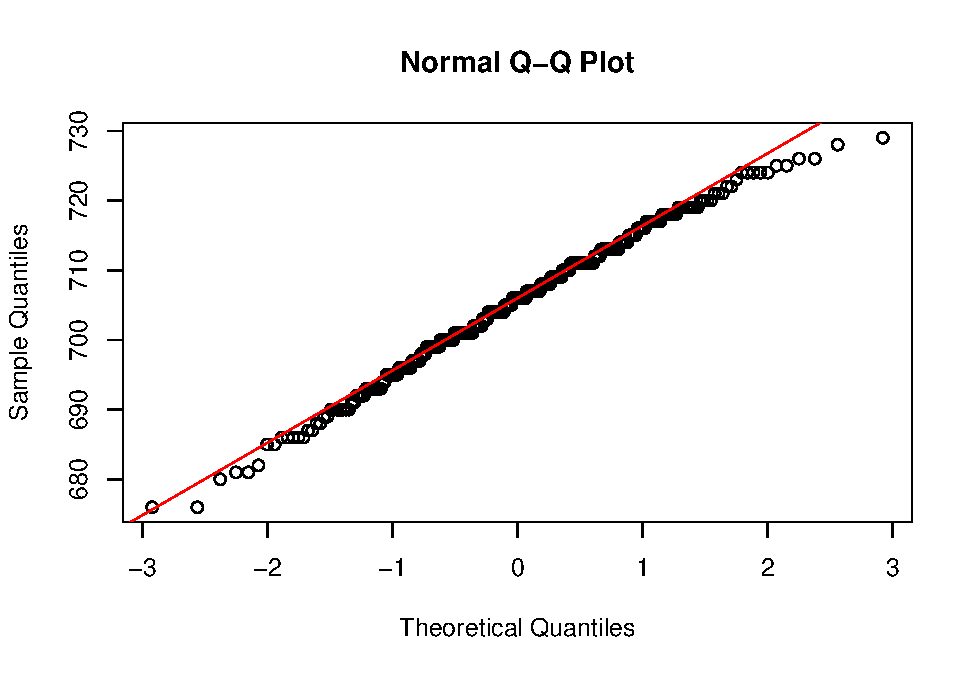
\includegraphics{EDA_files/figure-latex/unnamed-chunk-21-1.pdf}

Finally, boxplots summarize distributions visually:

\begin{Shaded}
\begin{Highlighting}[]
\FunctionTok{boxplot}\NormalTok{(old)}
\end{Highlighting}
\end{Shaded}

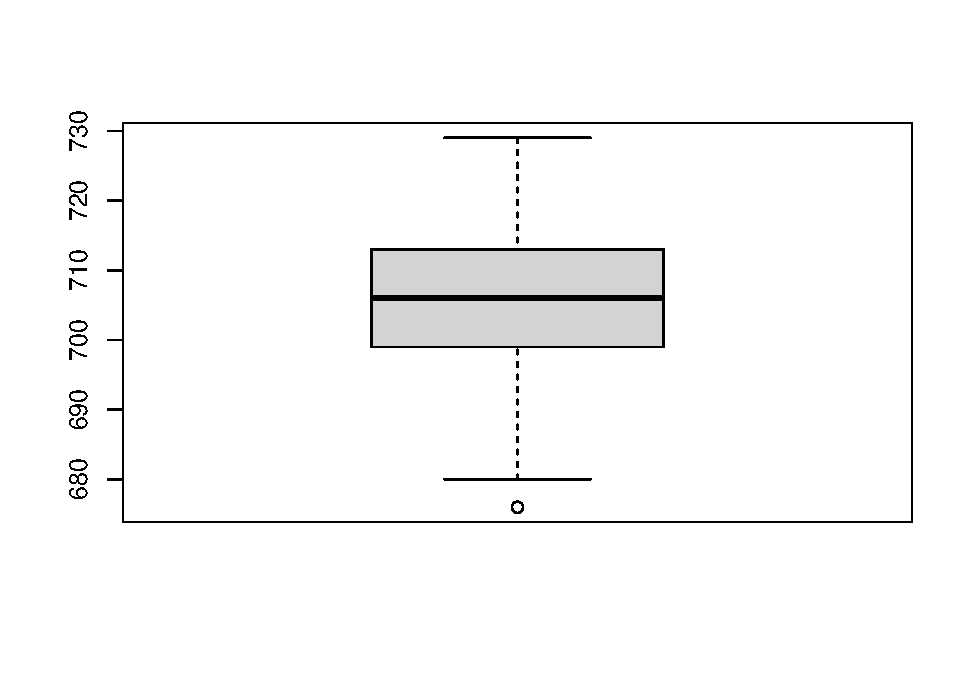
\includegraphics{EDA_files/figure-latex/unnamed-chunk-22-1.pdf}

The three horizontal lines that make up the box in a \textbf{boxplot}
represent the quartile values (from bottom to top: Q1, median, and Q3).
The outer lines (the ``whiskers'') indicate the minimum and maximum
values within a distance of \(1.5 \times \text{IQ}\) from the nearest
quartile, where \(\text{IQ}\) is the interquartile range. Any
observation outside this range is considered ``extreme,'' or an
\textbf{outlier}, and is represented separately. This type of
representation can be particularly useful when comparing two or more
distributions.

The primary role of the statistics calculated so far is to characterize
\textbf{location}, such as the mean and median, and \textbf{scale}, such
as the standard deviation and interquartile range. To these measures, we
can add \textbf{skewness} and \textbf{kurtosis}.

\hypertarget{skewness}{%
\paragraph{Skewness}\label{skewness}}

\textbf{Skewness} is a measure of symmetry, or more precisely, the lack
of symmetry in a distribution. A distribution is symmetric if it is
evenly distributed around its central point. For example, the standard
Gaussian distribution is symmetric around the mean \(\mu = 0\).

Given a sample \((Y_1, \ldots, Y_N)\), skewness can be calculated as:

\[
g_1 = \frac{\sum_{i=1}^N (Y_i - \bar{Y})^3 / N}{s^3}
\]

where \(\bar{Y}\) is the sample mean, \(s\) is the standard deviation,
and \(N\) is the number of observations. Note that here \(s\) is
calculated by dividing by \(N\) rather than \(N-1\). This formula is
known as the Fisher-Pearson coefficient of skewness. Some software also
implements an adjusted version:

\[
G_1 = \frac{\sqrt{N(N-1)}}{N-2} \cdot \frac{\sum_{i=1}^N (Y_i - \bar{Y})^3 / N}{s^3}
\]

The skewness of a normal distribution is 0, as is the case for any
symmetric distribution. Negative skewness indicates that the
observations are more concentrated on the left, while positive skewness
indicates a greater concentration on the right, with the right tail
being longer than the left.

\hypertarget{kurtosis}{%
\paragraph{Kurtosis}\label{kurtosis}}

\textbf{Kurtosis} compares the tails of a data distribution to those of
a normal distribution, providing information on whether the distribution
has heavier or lighter tails. The formula for kurtosis is:

\[
k_1 = \frac{\sum_{i=1}^N (Y_i - \bar{Y})^4 / N}{s^4}
\]

where \(\bar{Y}\) and \(s\) are the sample mean and standard deviation,
and \(N\) is the number of observations. Again, \(s\) is calculated by
dividing by \(N\). The kurtosis of the standard normal distribution is
3. Therefore, a more commonly used definition is:

\[
k_2 = \frac{\sum_{i=1}^N (Y_i - \bar{Y})^4 / N}{s^4} - 3
\]

This adjustment makes the kurtosis of the standard normal distribution
equal to 0. Positive values (\textit{heavy-tailed}) indicate that the
distribution has larger tails than a normal distribution, while negative
values (\textit{light-tailed}) indicate smaller tails.

\hypertarget{pre-processing}{%
\subsection{Pre-processing}\label{pre-processing}}

In practice, this step is generally very important and the most
time-consuming. This step includes: - formatting of variables type, and
consistent entrie; - dealing with \emph{missing values}; - dealing with
\emph{outliers}.

\hypertarget{what-is-an-outlier}{%
\subsubsection{What is an outlier?}\label{what-is-an-outlier}}

An \emph{outlier} is a value or an observation that is distant from
other observations, that is to say, a data point that differs
significantly from other data points. Alternatively, outliers can be
defined as observations not following the \emph{assumed model}, that is
values that deviate so much from other observations one might suppose a
different underlying sampling mechanism.

\hypertarget{how-to-detect-outliers-r}{%
\paragraph{How to detect outliers R?}\label{how-to-detect-outliers-r}}

\begin{itemize}
\tightlist
\item
  Descriptive statistics
\item
  Histogram
\item
  Boxplots
\item
  Percentiles
\end{itemize}

Outlier detection should be an important step during pre-processing,
that is the identification of observations which ``behave'' differently
with respect the majority of the data.\\
Sometimes outliers may be due to some errors (measurement, reporting,
\ldots) and then they can be discarded, substitued with \texttt{NA} (and
then apply a method able to handle \texttt{NA}), or substituted with an
\emph{estimate} of their value.\\
However, there is the possibility that these ``anomalous'' observations
underline a specific pattern in the data, and then should be included
and considered during the statistical analysis.

\hypertarget{what-is-a-missing-value}{%
\subsubsection{What is a missing value?}\label{what-is-a-missing-value}}

A missing value is one whose value is unknown. Missing values are
represented in R by the \texttt{NA} (not available) symbol. \texttt{NA}
is a special value whose properties are different from other values.\\
Missing values can be informative, understanding if the missing is due
to some reporting error or underline some specific pattern. One possible
option during pre-processing would be removing the entire observations
(rows) with at least one \texttt{NA}, or entire columns, if
\texttt{NA}'s occur only for specific variables.\\
\textbf{Remark}: In both cases we lose information, removing all the
related available data.\\
This may be a problem when our sample has few observations. An
alternative option is to consider methods, from the literature,
specifically designed for handling \texttt{NA}.

\hypertarget{example-the-penguins-data-set}{%
\subsection{Example: the Penguins data
set}\label{example-the-penguins-data-set}}

In this example, we consider the exploratory data analysis tools seen
before using the example \texttt{penguins} data set available in the
\texttt{palmerpenguins} package.

\begin{Shaded}
\begin{Highlighting}[]
\FunctionTok{library}\NormalTok{(palmerpenguins)}
\FunctionTok{data}\NormalTok{(}\StringTok{"penguins"}\NormalTok{)}
\end{Highlighting}
\end{Shaded}

Let's start displaying the structure and summary of the data set.

\begin{Shaded}
\begin{Highlighting}[]
\FunctionTok{str}\NormalTok{(penguins)}
\end{Highlighting}
\end{Shaded}

\begin{verbatim}
## tibble [344 x 8] (S3: tbl_df/tbl/data.frame)
##  $ species          : Factor w/ 3 levels "Adelie","Chinstrap",..: 1 1 1 1 1 1 1 1 1 1 ...
##  $ island           : Factor w/ 3 levels "Biscoe","Dream",..: 3 3 3 3 3 3 3 3 3 3 ...
##  $ bill_length_mm   : num [1:344] 39.1 39.5 40.3 NA 36.7 39.3 38.9 39.2 34.1 42 ...
##  $ bill_depth_mm    : num [1:344] 18.7 17.4 18 NA 19.3 20.6 17.8 19.6 18.1 20.2 ...
##  $ flipper_length_mm: int [1:344] 181 186 195 NA 193 190 181 195 193 190 ...
##  $ body_mass_g      : int [1:344] 3750 3800 3250 NA 3450 3650 3625 4675 3475 4250 ...
##  $ sex              : Factor w/ 2 levels "female","male": 2 1 1 NA 1 2 1 2 NA NA ...
##  $ year             : int [1:344] 2007 2007 2007 2007 2007 2007 2007 2007 2007 2007 ...
\end{verbatim}

\begin{Shaded}
\begin{Highlighting}[]
\FunctionTok{summary}\NormalTok{(penguins)}
\end{Highlighting}
\end{Shaded}

\begin{verbatim}
##       species          island    bill_length_mm  bill_depth_mm  
##  Adelie   :152   Biscoe   :168   Min.   :32.10   Min.   :13.10  
##  Chinstrap: 68   Dream    :124   1st Qu.:39.23   1st Qu.:15.60  
##  Gentoo   :124   Torgersen: 52   Median :44.45   Median :17.30  
##                                  Mean   :43.92   Mean   :17.15  
##                                  3rd Qu.:48.50   3rd Qu.:18.70  
##                                  Max.   :59.60   Max.   :21.50  
##                                  NA's   :2       NA's   :2      
##  flipper_length_mm  body_mass_g       sex           year     
##  Min.   :172.0     Min.   :2700   female:165   Min.   :2007  
##  1st Qu.:190.0     1st Qu.:3550   male  :168   1st Qu.:2007  
##  Median :197.0     Median :4050   NA's  : 11   Median :2008  
##  Mean   :200.9     Mean   :4202                Mean   :2008  
##  3rd Qu.:213.0     3rd Qu.:4750                3rd Qu.:2009  
##  Max.   :231.0     Max.   :6300                Max.   :2009  
##  NA's   :2         NA's   :2
\end{verbatim}

There are some missing values in the data set. As first step we can
identfy the observations which contain NA values.

\begin{Shaded}
\begin{Highlighting}[]
\NormalTok{penguins }\SpecialCharTok{\%\textgreater{}\%} \FunctionTok{filter}\NormalTok{(}\FunctionTok{is.na}\NormalTok{(sex))}
\end{Highlighting}
\end{Shaded}

\begin{verbatim}
## # A tibble: 11 x 8
##    species island    bill_length_mm bill_depth_mm flipper_length_mm body_mass_g
##    <fct>   <fct>              <dbl>         <dbl>             <int>       <int>
##  1 Adelie  Torgersen           NA            NA                  NA          NA
##  2 Adelie  Torgersen           34.1          18.1               193        3475
##  3 Adelie  Torgersen           42            20.2               190        4250
##  4 Adelie  Torgersen           37.8          17.1               186        3300
##  5 Adelie  Torgersen           37.8          17.3               180        3700
##  6 Adelie  Dream               37.5          18.9               179        2975
##  7 Gentoo  Biscoe              44.5          14.3               216        4100
##  8 Gentoo  Biscoe              46.2          14.4               214        4650
##  9 Gentoo  Biscoe              47.3          13.8               216        4725
## 10 Gentoo  Biscoe              44.5          15.7               217        4875
## 11 Gentoo  Biscoe              NA            NA                  NA          NA
## # i 2 more variables: sex <fct>, year <int>
\end{verbatim}

There are 2 observations with missing sex, bill length, bill depth,
flipper length and body mass. We can remove them.\\
There are additional 9 observations with missing value only in the sex
variable. These observations could be maintained for the analysis that
don't include sex. However, for this example we will remove all 11 rows.

\begin{Shaded}
\begin{Highlighting}[]
\NormalTok{peng\_data }\OtherTok{\textless{}{-}}\NormalTok{ penguins }\SpecialCharTok{\%\textgreater{}\%} \FunctionTok{filter}\NormalTok{(}\SpecialCharTok{!}\FunctionTok{is.na}\NormalTok{(sex))}
\FunctionTok{summary}\NormalTok{(peng\_data)}
\end{Highlighting}
\end{Shaded}

\begin{verbatim}
##       species          island    bill_length_mm  bill_depth_mm  
##  Adelie   :146   Biscoe   :163   Min.   :32.10   Min.   :13.10  
##  Chinstrap: 68   Dream    :123   1st Qu.:39.50   1st Qu.:15.60  
##  Gentoo   :119   Torgersen: 47   Median :44.50   Median :17.30  
##                                  Mean   :43.99   Mean   :17.16  
##                                  3rd Qu.:48.60   3rd Qu.:18.70  
##                                  Max.   :59.60   Max.   :21.50  
##  flipper_length_mm  body_mass_g       sex           year     
##  Min.   :172       Min.   :2700   female:165   Min.   :2007  
##  1st Qu.:190       1st Qu.:3550   male  :168   1st Qu.:2007  
##  Median :197       Median :4050                Median :2008  
##  Mean   :201       Mean   :4207                Mean   :2008  
##  3rd Qu.:213       3rd Qu.:4775                3rd Qu.:2009  
##  Max.   :231       Max.   :6300                Max.   :2009
\end{verbatim}

We can explore the variables singularly.

For the discrete variables, we can display the frequencies

\begin{Shaded}
\begin{Highlighting}[]
\NormalTok{p1 }\OtherTok{\textless{}{-}} \FunctionTok{ggplot}\NormalTok{(}\AttributeTok{data =}\NormalTok{ peng\_data, }\AttributeTok{mapping =} \FunctionTok{aes}\NormalTok{(}\AttributeTok{x =}\NormalTok{ species)) }\SpecialCharTok{+} 
  \FunctionTok{geom\_bar}\NormalTok{(}\AttributeTok{fill =}  \StringTok{"green"}\NormalTok{)}

\NormalTok{p2 }\OtherTok{\textless{}{-}} \FunctionTok{ggplot}\NormalTok{(}\AttributeTok{data =}\NormalTok{ peng\_data, }\AttributeTok{mapping =} \FunctionTok{aes}\NormalTok{(}\AttributeTok{x =}\NormalTok{ island)) }\SpecialCharTok{+} 
  \FunctionTok{geom\_bar}\NormalTok{(}\AttributeTok{fill=} \StringTok{"blue"}\NormalTok{)}

\NormalTok{p3 }\OtherTok{\textless{}{-}} \FunctionTok{ggplot}\NormalTok{(}\AttributeTok{data =}\NormalTok{ peng\_data, }\AttributeTok{mapping =} \FunctionTok{aes}\NormalTok{(}\AttributeTok{x =}\NormalTok{ sex)) }\SpecialCharTok{+} 
  \FunctionTok{geom\_bar}\NormalTok{( }\AttributeTok{fill=} \StringTok{"purple"}\NormalTok{)}

\NormalTok{p4 }\OtherTok{\textless{}{-}} \FunctionTok{ggplot}\NormalTok{(}\AttributeTok{data =}\NormalTok{ peng\_data, }\AttributeTok{mapping =} \FunctionTok{aes}\NormalTok{(}\AttributeTok{x =}\NormalTok{ year)) }\SpecialCharTok{+} 
  \FunctionTok{geom\_bar}\NormalTok{(}\AttributeTok{fill=} \StringTok{"orange"}\NormalTok{)}

\NormalTok{gridExtra}\SpecialCharTok{::}\FunctionTok{grid.arrange}\NormalTok{(p1,p2,p3,p4, }\AttributeTok{nrow=}\DecValTok{2}\NormalTok{)}
\end{Highlighting}
\end{Shaded}

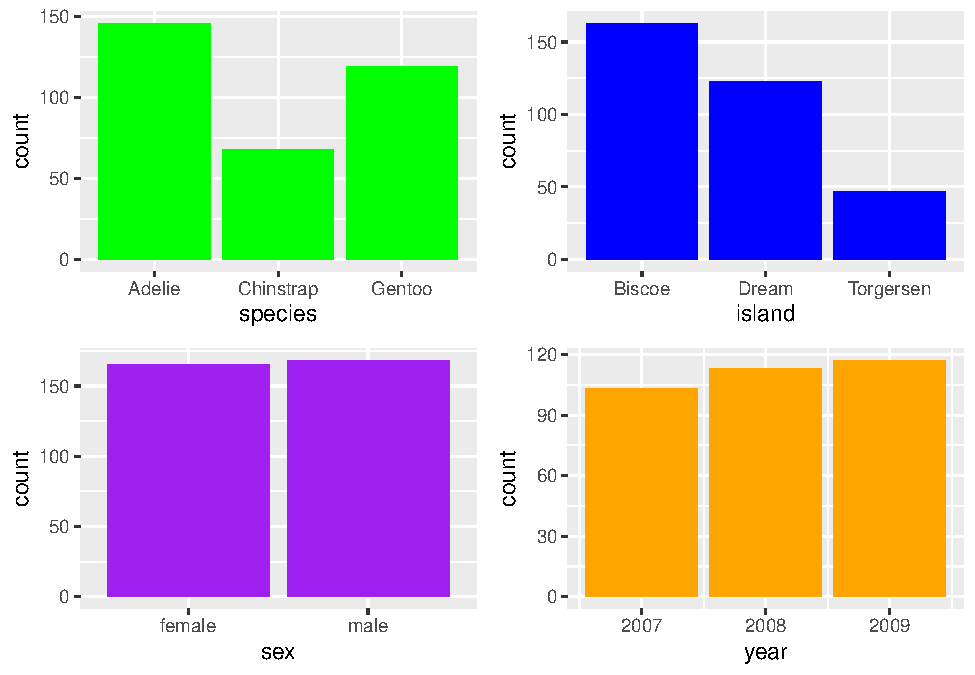
\includegraphics{EDA_files/figure-latex/unnamed-chunk-27-1.pdf}

or we can combine information

\begin{Shaded}
\begin{Highlighting}[]
\NormalTok{p1 }\OtherTok{\textless{}{-}} \FunctionTok{ggplot}\NormalTok{(}\AttributeTok{data =}\NormalTok{ peng\_data, }\AttributeTok{mapping =} \FunctionTok{aes}\NormalTok{(}\AttributeTok{x =}\NormalTok{ species, }\AttributeTok{fill =}\NormalTok{  island)) }\SpecialCharTok{+} 
  \FunctionTok{geom\_bar}\NormalTok{()}

\NormalTok{p2 }\OtherTok{\textless{}{-}} \FunctionTok{ggplot}\NormalTok{(}\AttributeTok{data =}\NormalTok{ peng\_data, }\AttributeTok{mapping =} \FunctionTok{aes}\NormalTok{(}\AttributeTok{x =}\NormalTok{ island, }\AttributeTok{fill=}\NormalTok{ sex)) }\SpecialCharTok{+} 
  \FunctionTok{geom\_bar}\NormalTok{()}

\NormalTok{p3 }\OtherTok{\textless{}{-}} \FunctionTok{ggplot}\NormalTok{(}\AttributeTok{data =}\NormalTok{ peng\_data, }\AttributeTok{mapping =} \FunctionTok{aes}\NormalTok{(}\AttributeTok{x =}\NormalTok{ species, }\AttributeTok{fill=}\NormalTok{ sex)) }\SpecialCharTok{+} 
  \FunctionTok{geom\_bar}\NormalTok{()}

\NormalTok{gridExtra}\SpecialCharTok{::}\FunctionTok{grid.arrange}\NormalTok{(p2,p3,p1, }\AttributeTok{nrow=}\DecValTok{2}\NormalTok{)}
\end{Highlighting}
\end{Shaded}

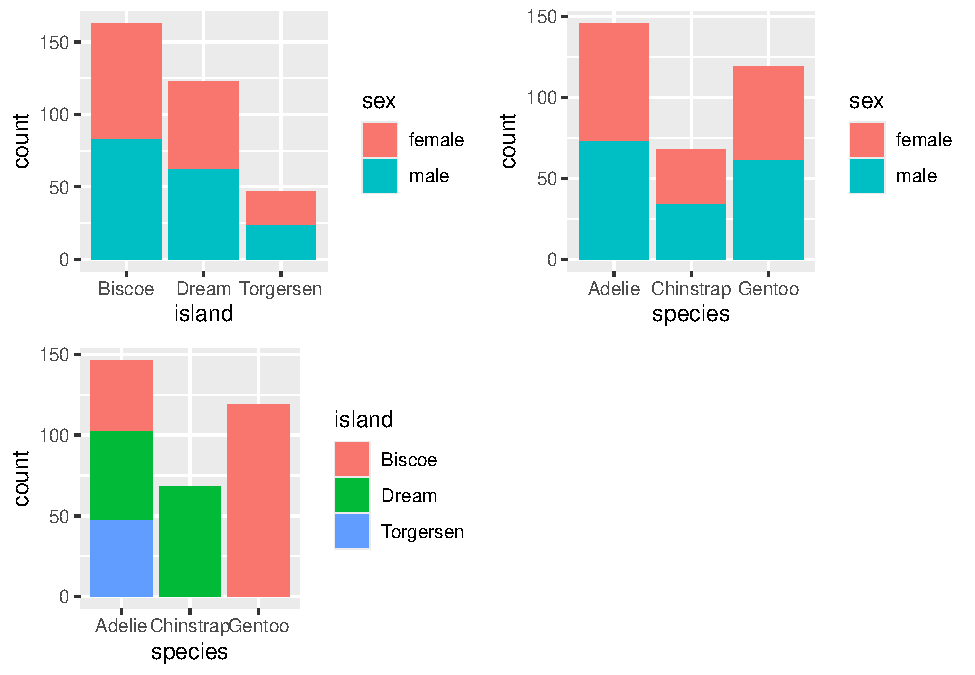
\includegraphics{EDA_files/figure-latex/unnamed-chunk-28-1.pdf}

Equivalently we can display the relative frequencies.\\
For the continuous variables, we can explore the single distributions
using the histograms

\begin{Shaded}
\begin{Highlighting}[]
\NormalTok{p1 }\OtherTok{\textless{}{-}} \FunctionTok{ggplot}\NormalTok{(}\AttributeTok{data =}\NormalTok{ peng\_data, }\AttributeTok{mapping =} \FunctionTok{aes}\NormalTok{(}\AttributeTok{x =}\NormalTok{ bill\_length\_mm)) }\SpecialCharTok{+} 
  \FunctionTok{geom\_histogram}\NormalTok{(}\AttributeTok{fill =}  \StringTok{"green"}\NormalTok{, }\AttributeTok{bins =} \DecValTok{40}\NormalTok{)}

\NormalTok{p2 }\OtherTok{\textless{}{-}} \FunctionTok{ggplot}\NormalTok{(}\AttributeTok{data =}\NormalTok{ peng\_data, }\AttributeTok{mapping =} \FunctionTok{aes}\NormalTok{(}\AttributeTok{x =}\NormalTok{ bill\_depth\_mm)) }\SpecialCharTok{+} 
  \FunctionTok{geom\_histogram}\NormalTok{(}\AttributeTok{fill=} \StringTok{"blue"}\NormalTok{, }\AttributeTok{bins =} \DecValTok{40}\NormalTok{)}

\NormalTok{p3 }\OtherTok{\textless{}{-}} \FunctionTok{ggplot}\NormalTok{(}\AttributeTok{data =}\NormalTok{ peng\_data, }\AttributeTok{mapping =} \FunctionTok{aes}\NormalTok{(}\AttributeTok{x =}\NormalTok{ flipper\_length\_mm)) }\SpecialCharTok{+} 
  \FunctionTok{geom\_histogram}\NormalTok{( }\AttributeTok{fill=} \StringTok{"purple"}\NormalTok{, }\AttributeTok{bins =} \DecValTok{40}\NormalTok{)}

\NormalTok{p4 }\OtherTok{\textless{}{-}} \FunctionTok{ggplot}\NormalTok{(}\AttributeTok{data =}\NormalTok{ peng\_data, }\AttributeTok{mapping =} \FunctionTok{aes}\NormalTok{(}\AttributeTok{x =}\NormalTok{ body\_mass\_g)) }\SpecialCharTok{+} 
  \FunctionTok{geom\_histogram}\NormalTok{(}\AttributeTok{fill=} \StringTok{"orange"}\NormalTok{, }\AttributeTok{bins =} \DecValTok{40}\NormalTok{)}

\NormalTok{gridExtra}\SpecialCharTok{::}\FunctionTok{grid.arrange}\NormalTok{(p1,p2,p3,p4, }\AttributeTok{nrow=}\DecValTok{2}\NormalTok{)}
\end{Highlighting}
\end{Shaded}

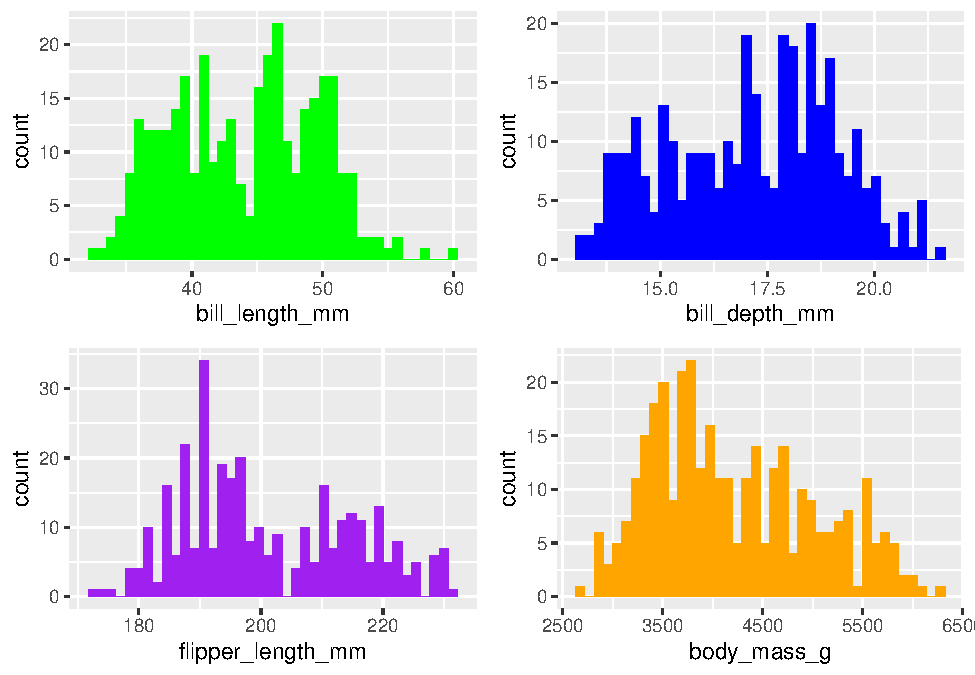
\includegraphics{EDA_files/figure-latex/unnamed-chunk-29-1.pdf}

The histograms show multimodal distributions for the considered
variables. We can have additional information by considering the
\texttt{species}

\begin{Shaded}
\begin{Highlighting}[]
\NormalTok{p1 }\OtherTok{\textless{}{-}} \FunctionTok{ggplot}\NormalTok{(}\AttributeTok{data =}\NormalTok{ peng\_data, }\AttributeTok{mapping =} \FunctionTok{aes}\NormalTok{(}\AttributeTok{x =}\NormalTok{ bill\_length\_mm, }\AttributeTok{color=}\NormalTok{species, }\AttributeTok{fill =}\NormalTok{  species)) }\SpecialCharTok{+} 
  \FunctionTok{geom\_histogram}\NormalTok{( }\AttributeTok{bins =} \DecValTok{40}\NormalTok{)}

\NormalTok{p2 }\OtherTok{\textless{}{-}} \FunctionTok{ggplot}\NormalTok{(}\AttributeTok{data =}\NormalTok{ peng\_data, }\AttributeTok{mapping =} \FunctionTok{aes}\NormalTok{(}\AttributeTok{x =}\NormalTok{ bill\_depth\_mm, }\AttributeTok{fill =}\NormalTok{  species)) }\SpecialCharTok{+} 
  \FunctionTok{geom\_histogram}\NormalTok{(}\AttributeTok{bins =} \DecValTok{40}\NormalTok{)}

\NormalTok{p3 }\OtherTok{\textless{}{-}} \FunctionTok{ggplot}\NormalTok{(}\AttributeTok{data =}\NormalTok{ peng\_data, }\AttributeTok{mapping =} \FunctionTok{aes}\NormalTok{(}\AttributeTok{x =}\NormalTok{ flipper\_length\_mm, }\AttributeTok{color=}\NormalTok{species, }\AttributeTok{fill =}\NormalTok{  species)) }\SpecialCharTok{+} 
  \FunctionTok{geom\_histogram}\NormalTok{( }\AttributeTok{bins =} \DecValTok{40}\NormalTok{)}

\NormalTok{p4 }\OtherTok{\textless{}{-}} \FunctionTok{ggplot}\NormalTok{(}\AttributeTok{data =}\NormalTok{ peng\_data, }\AttributeTok{mapping =} \FunctionTok{aes}\NormalTok{(}\AttributeTok{x =}\NormalTok{ body\_mass\_g, }\AttributeTok{color=}\NormalTok{species, }\AttributeTok{fill =}\NormalTok{  species)) }\SpecialCharTok{+} 
  \FunctionTok{geom\_histogram}\NormalTok{(}\AttributeTok{bins =} \DecValTok{40}\NormalTok{)}

\NormalTok{gridExtra}\SpecialCharTok{::}\FunctionTok{grid.arrange}\NormalTok{(p1,p2,p3,p4, }\AttributeTok{nrow=}\DecValTok{2}\NormalTok{)}
\end{Highlighting}
\end{Shaded}

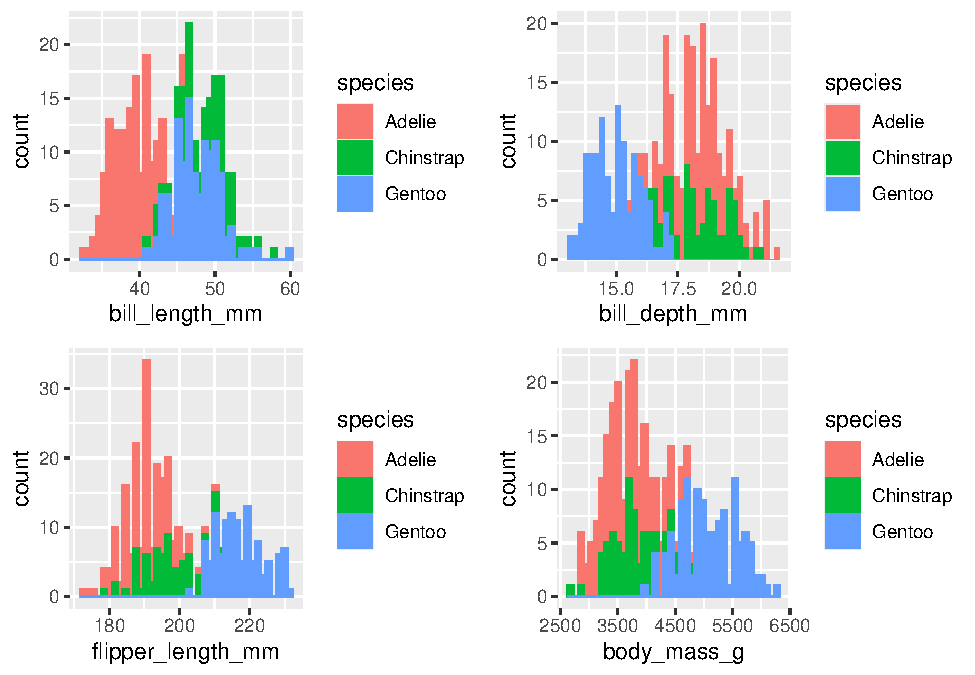
\includegraphics{EDA_files/figure-latex/unnamed-chunk-30-1.pdf}

Alternatively we can show the estimated density

\begin{Shaded}
\begin{Highlighting}[]
\FunctionTok{ggplot}\NormalTok{(}\AttributeTok{data =}\NormalTok{ peng\_data, }\FunctionTok{aes}\NormalTok{(}\AttributeTok{x =}\NormalTok{ bill\_length\_mm, }\AttributeTok{color =}\NormalTok{ species)) }\SpecialCharTok{+} 
  \FunctionTok{geom\_density}\NormalTok{(}\AttributeTok{size=}\DecValTok{1}\NormalTok{) }\SpecialCharTok{+}
  \FunctionTok{geom\_histogram}\NormalTok{(}\FunctionTok{aes}\NormalTok{(}\AttributeTok{y =} \FunctionTok{after\_stat}\NormalTok{(density),}\AttributeTok{fill =}\NormalTok{  species), }\AttributeTok{bins =} \DecValTok{40}\NormalTok{, }\AttributeTok{alpha=}\FloatTok{0.3}\NormalTok{) }\SpecialCharTok{+}
  \FunctionTok{theme\_classic}\NormalTok{()}
\end{Highlighting}
\end{Shaded}

\begin{verbatim}
## Warning: Using `size` aesthetic for lines was deprecated in ggplot2 3.4.0.
## i Please use `linewidth` instead.
## This warning is displayed once every 8 hours.
## Call `lifecycle::last_lifecycle_warnings()` to see where this warning was
## generated.
\end{verbatim}

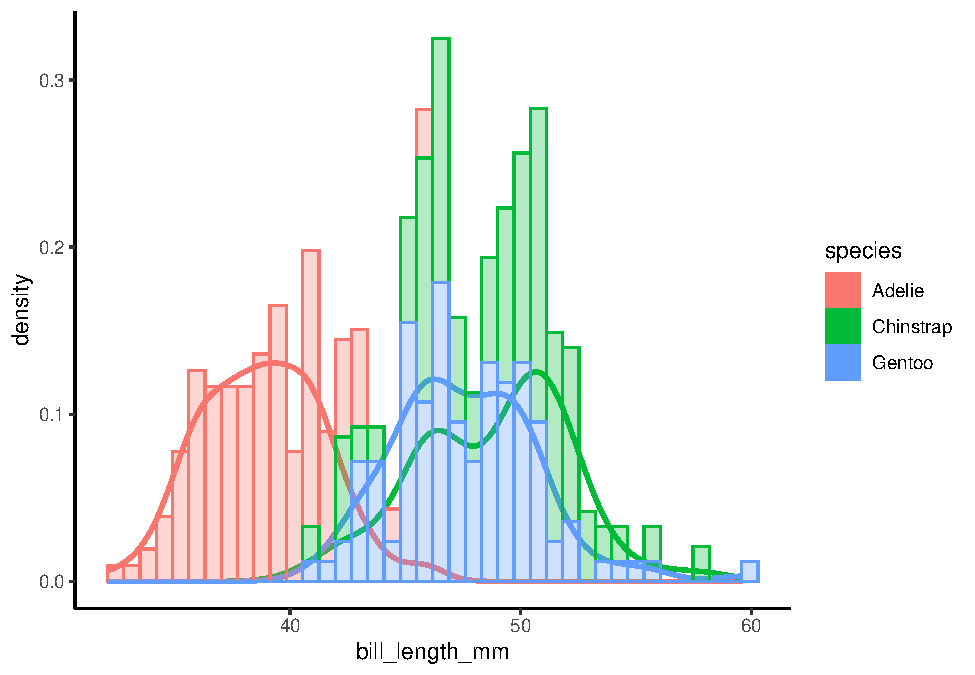
\includegraphics{EDA_files/figure-latex/unnamed-chunk-31-1.pdf}

The distribution of observations from a continuous random variable can
be also displayed using the boxplot

\begin{Shaded}
\begin{Highlighting}[]
\FunctionTok{ggplot}\NormalTok{(}\AttributeTok{data =}\NormalTok{ peng\_data, }\FunctionTok{aes}\NormalTok{(}\AttributeTok{y =}\NormalTok{ bill\_length\_mm, }\AttributeTok{fill =}\NormalTok{ species)) }\SpecialCharTok{+} 
  \FunctionTok{geom\_boxplot}\NormalTok{() }\SpecialCharTok{+}
  \FunctionTok{theme\_classic}\NormalTok{()}
\end{Highlighting}
\end{Shaded}

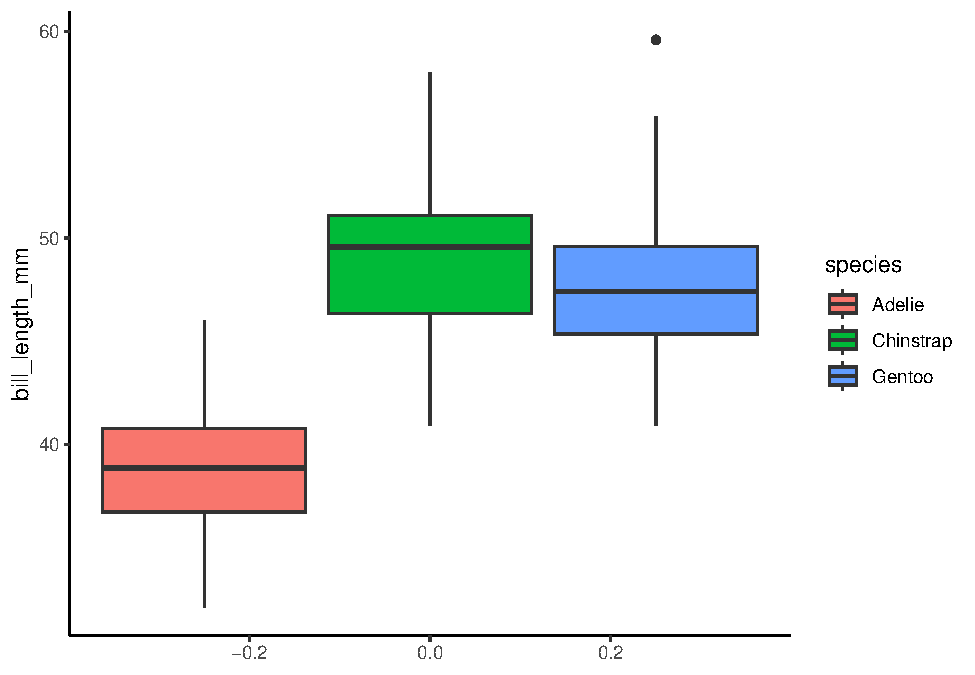
\includegraphics{EDA_files/figure-latex/unnamed-chunk-32-1.pdf}

We can study the relationship between pairs of continuous variables
using the scatter-plot

\begin{Shaded}
\begin{Highlighting}[]
\NormalTok{p1 }\OtherTok{\textless{}{-}} \FunctionTok{ggplot}\NormalTok{(peng\_data, }\FunctionTok{aes}\NormalTok{(}\AttributeTok{x=}\NormalTok{bill\_length\_mm, }\AttributeTok{y=}\NormalTok{bill\_depth\_mm)) }\SpecialCharTok{+}
  \FunctionTok{geom\_point}\NormalTok{()}
\NormalTok{p2 }\OtherTok{\textless{}{-}} \FunctionTok{ggplot}\NormalTok{(peng\_data, }\FunctionTok{aes}\NormalTok{(}\AttributeTok{x=}\NormalTok{bill\_length\_mm, }\AttributeTok{y=}\NormalTok{flipper\_length\_mm)) }\SpecialCharTok{+}
  \FunctionTok{geom\_point}\NormalTok{()}
\NormalTok{p3 }\OtherTok{\textless{}{-}} \FunctionTok{ggplot}\NormalTok{(peng\_data, }\FunctionTok{aes}\NormalTok{(}\AttributeTok{x=}\NormalTok{bill\_length\_mm, }\AttributeTok{y=}\NormalTok{body\_mass\_g)) }\SpecialCharTok{+}
  \FunctionTok{geom\_point}\NormalTok{()}
\NormalTok{p4 }\OtherTok{\textless{}{-}} \FunctionTok{ggplot}\NormalTok{(peng\_data, }\FunctionTok{aes}\NormalTok{(}\AttributeTok{x=}\NormalTok{bill\_depth\_mm, }\AttributeTok{y=}\NormalTok{flipper\_length\_mm)) }\SpecialCharTok{+}
  \FunctionTok{geom\_point}\NormalTok{()}
\NormalTok{p5 }\OtherTok{\textless{}{-}} \FunctionTok{ggplot}\NormalTok{(peng\_data, }\FunctionTok{aes}\NormalTok{(}\AttributeTok{x=}\NormalTok{bill\_depth\_mm, }\AttributeTok{y=}\NormalTok{body\_mass\_g)) }\SpecialCharTok{+}
  \FunctionTok{geom\_point}\NormalTok{()}
\NormalTok{p6 }\OtherTok{\textless{}{-}} \FunctionTok{ggplot}\NormalTok{(peng\_data, }\FunctionTok{aes}\NormalTok{(}\AttributeTok{x=}\NormalTok{flipper\_length\_mm, }\AttributeTok{y=}\NormalTok{body\_mass\_g)) }\SpecialCharTok{+}
  \FunctionTok{geom\_point}\NormalTok{()}
\NormalTok{gridExtra}\SpecialCharTok{::}\FunctionTok{grid.arrange}\NormalTok{(p1, p2, p3,p4, p5, p6, }\AttributeTok{nrow=}\DecValTok{2}\NormalTok{)}
\end{Highlighting}
\end{Shaded}

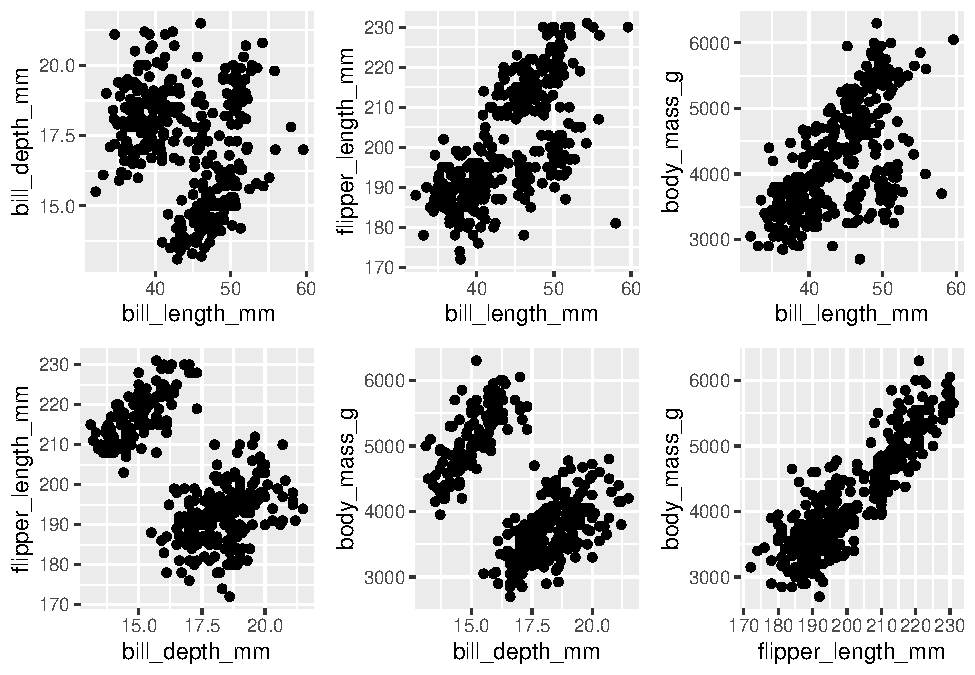
\includegraphics{EDA_files/figure-latex/unnamed-chunk-33-1.pdf}

We can see that data points show different patterns. We can color data
points by the species

\begin{Shaded}
\begin{Highlighting}[]
\NormalTok{p1 }\OtherTok{\textless{}{-}} \FunctionTok{ggplot}\NormalTok{(peng\_data, }\FunctionTok{aes}\NormalTok{(}\AttributeTok{x=}\NormalTok{bill\_length\_mm, }\AttributeTok{y=}\NormalTok{bill\_depth\_mm, }\AttributeTok{color=}\NormalTok{species)) }\SpecialCharTok{+}
  \FunctionTok{geom\_point}\NormalTok{()}
\NormalTok{p2 }\OtherTok{\textless{}{-}} \FunctionTok{ggplot}\NormalTok{(peng\_data, }\FunctionTok{aes}\NormalTok{(}\AttributeTok{x=}\NormalTok{bill\_length\_mm, }\AttributeTok{y=}\NormalTok{flipper\_length\_mm, }\AttributeTok{color=}\NormalTok{species)) }\SpecialCharTok{+}
  \FunctionTok{geom\_point}\NormalTok{()}
\NormalTok{p3 }\OtherTok{\textless{}{-}} \FunctionTok{ggplot}\NormalTok{(peng\_data, }\FunctionTok{aes}\NormalTok{(}\AttributeTok{x=}\NormalTok{bill\_length\_mm, }\AttributeTok{y=}\NormalTok{body\_mass\_g, }\AttributeTok{color=}\NormalTok{species)) }\SpecialCharTok{+}
  \FunctionTok{geom\_point}\NormalTok{()}
\NormalTok{p4 }\OtherTok{\textless{}{-}} \FunctionTok{ggplot}\NormalTok{(peng\_data, }\FunctionTok{aes}\NormalTok{(}\AttributeTok{x=}\NormalTok{bill\_depth\_mm, }\AttributeTok{y=}\NormalTok{flipper\_length\_mm, }\AttributeTok{color=}\NormalTok{species)) }\SpecialCharTok{+}
  \FunctionTok{geom\_point}\NormalTok{()}
\NormalTok{p5 }\OtherTok{\textless{}{-}} \FunctionTok{ggplot}\NormalTok{(peng\_data, }\FunctionTok{aes}\NormalTok{(}\AttributeTok{x=}\NormalTok{bill\_depth\_mm, }\AttributeTok{y=}\NormalTok{body\_mass\_g, }\AttributeTok{color=}\NormalTok{species)) }\SpecialCharTok{+}
  \FunctionTok{geom\_point}\NormalTok{()}
\NormalTok{p6 }\OtherTok{\textless{}{-}} \FunctionTok{ggplot}\NormalTok{(peng\_data, }\FunctionTok{aes}\NormalTok{(}\AttributeTok{x=}\NormalTok{flipper\_length\_mm, }\AttributeTok{y=}\NormalTok{body\_mass\_g, }\AttributeTok{color=}\NormalTok{species)) }\SpecialCharTok{+}
  \FunctionTok{geom\_point}\NormalTok{()}
\NormalTok{gridExtra}\SpecialCharTok{::}\FunctionTok{grid.arrange}\NormalTok{(p1, p2, p3,p4, p5, p6, }\AttributeTok{nrow=}\DecValTok{3}\NormalTok{)}
\end{Highlighting}
\end{Shaded}

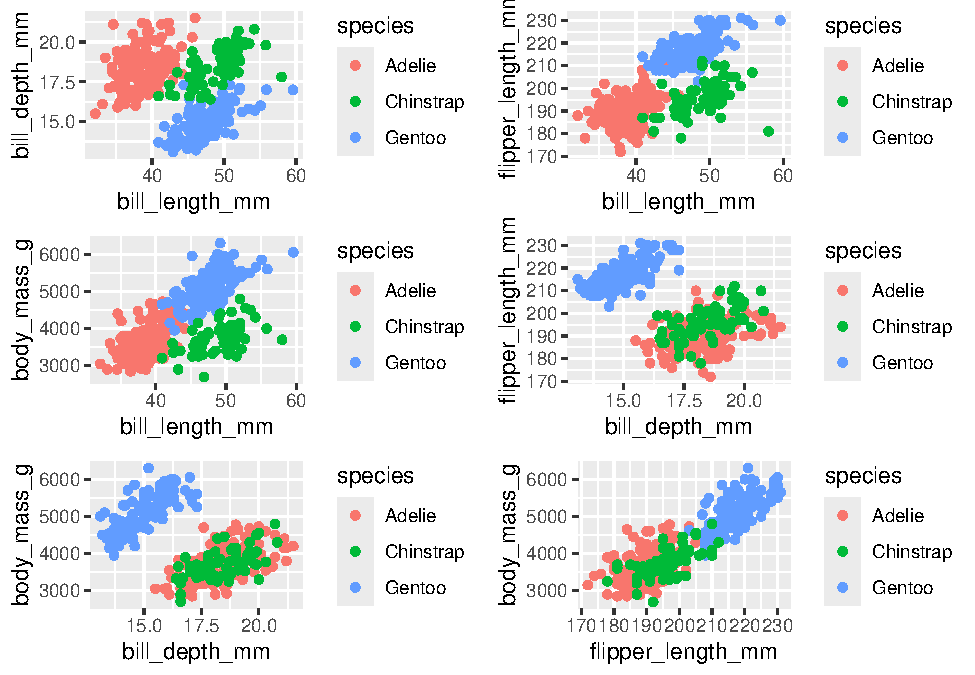
\includegraphics{EDA_files/figure-latex/unnamed-chunk-34-1.pdf}

We could add also the island and/or sex information to the same plot

\begin{Shaded}
\begin{Highlighting}[]
\FunctionTok{ggplot}\NormalTok{(peng\_data, }\FunctionTok{aes}\NormalTok{(}\AttributeTok{x=}\NormalTok{bill\_length\_mm, }\AttributeTok{y=}\NormalTok{bill\_depth\_mm, }\AttributeTok{color=}\NormalTok{species)) }\SpecialCharTok{+}
  \FunctionTok{geom\_point}\NormalTok{(}\FunctionTok{aes}\NormalTok{(}\AttributeTok{shape=}\NormalTok{sex))}\SpecialCharTok{+}
  \FunctionTok{facet\_wrap}\NormalTok{(.}\SpecialCharTok{\textasciitilde{}}\NormalTok{island)}
\end{Highlighting}
\end{Shaded}

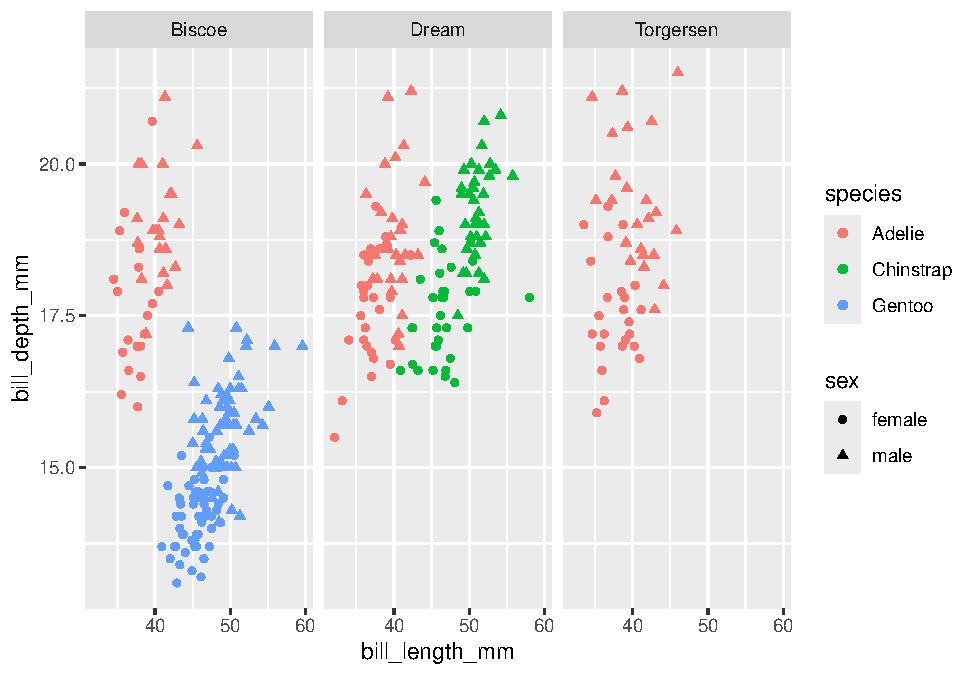
\includegraphics{EDA_files/figure-latex/unnamed-chunk-35-1.pdf}

\textbf{Remark}: Plots with several levels of information can be very
useful when exploring the data set, since they allow to have a general
view of the data set and the relations among variables. On the other
hand, when showing results they could appear unclear or overwhelming.
Think carefully on the aspect of the data set that you want to explore
or show, then create specific plots.

Finally, we consider the correlation among variables

\begin{Shaded}
\begin{Highlighting}[]
\NormalTok{corr\_matrix }\OtherTok{\textless{}{-}} \FunctionTok{round}\NormalTok{(}\FunctionTok{cor}\NormalTok{(peng\_data[,}\DecValTok{3}\SpecialCharTok{:}\DecValTok{6}\NormalTok{]), }\DecValTok{2}\NormalTok{)}
\NormalTok{corr\_matrix}
\end{Highlighting}
\end{Shaded}

\begin{verbatim}
##                   bill_length_mm bill_depth_mm flipper_length_mm body_mass_g
## bill_length_mm              1.00         -0.23              0.65        0.59
## bill_depth_mm              -0.23          1.00             -0.58       -0.47
## flipper_length_mm           0.65         -0.58              1.00        0.87
## body_mass_g                 0.59         -0.47              0.87        1.00
\end{verbatim}

\begin{Shaded}
\begin{Highlighting}[]
\FunctionTok{library}\NormalTok{(ggcorrplot)                                             }
\end{Highlighting}
\end{Shaded}

\begin{verbatim}
## Warning: il pacchetto 'ggcorrplot' è stato creato con R versione 4.3.3
\end{verbatim}

\begin{Shaded}
\begin{Highlighting}[]
\FunctionTok{ggcorrplot}\NormalTok{(corr\_matrix, }
           \AttributeTok{type =} \StringTok{"upper"}\NormalTok{, }
           \AttributeTok{lab =}\NormalTok{ T, }
           \AttributeTok{lab\_size =} \DecValTok{7}\NormalTok{, }
           \AttributeTok{outline.col =} \StringTok{"white"}\NormalTok{, }
           \AttributeTok{colors =} \FunctionTok{c}\NormalTok{(}\StringTok{"tomato2"}\NormalTok{, }\StringTok{"white"}\NormalTok{, }\StringTok{"springgreen3"}\NormalTok{), }
           \AttributeTok{title =} \StringTok{""}\NormalTok{, }
           \AttributeTok{ggtheme =}\NormalTok{ theme\_gray, }
           \AttributeTok{pch.cex =} \DecValTok{30}\NormalTok{, }
           \AttributeTok{tl.cex =} \DecValTok{20}\NormalTok{)}
\end{Highlighting}
\end{Shaded}

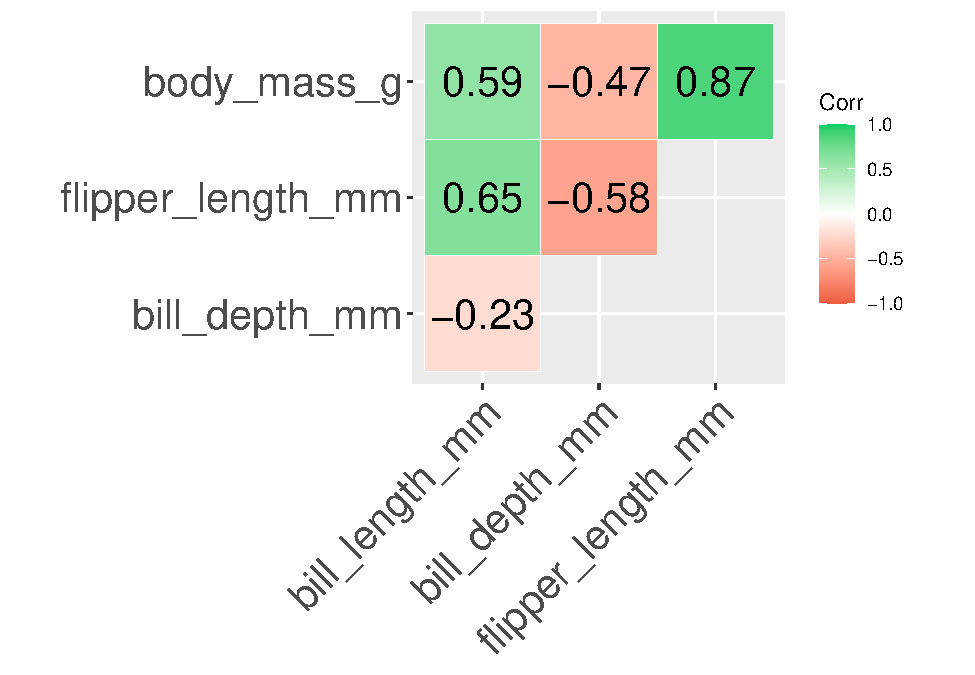
\includegraphics{EDA_files/figure-latex/unnamed-chunk-36-1.pdf}

A fast way for visualizing all these plots at once is provided by the
function \texttt{ggpairs} in the \texttt{GGally} package

\begin{Shaded}
\begin{Highlighting}[]
\FunctionTok{library}\NormalTok{(GGally)}
\FunctionTok{ggpairs}\NormalTok{(peng\_data[,}\FunctionTok{c}\NormalTok{(}\DecValTok{1}\NormalTok{,}\DecValTok{3}\SpecialCharTok{:}\DecValTok{6}\NormalTok{)], }\FunctionTok{aes}\NormalTok{(}\AttributeTok{color=}\NormalTok{species))}
\end{Highlighting}
\end{Shaded}

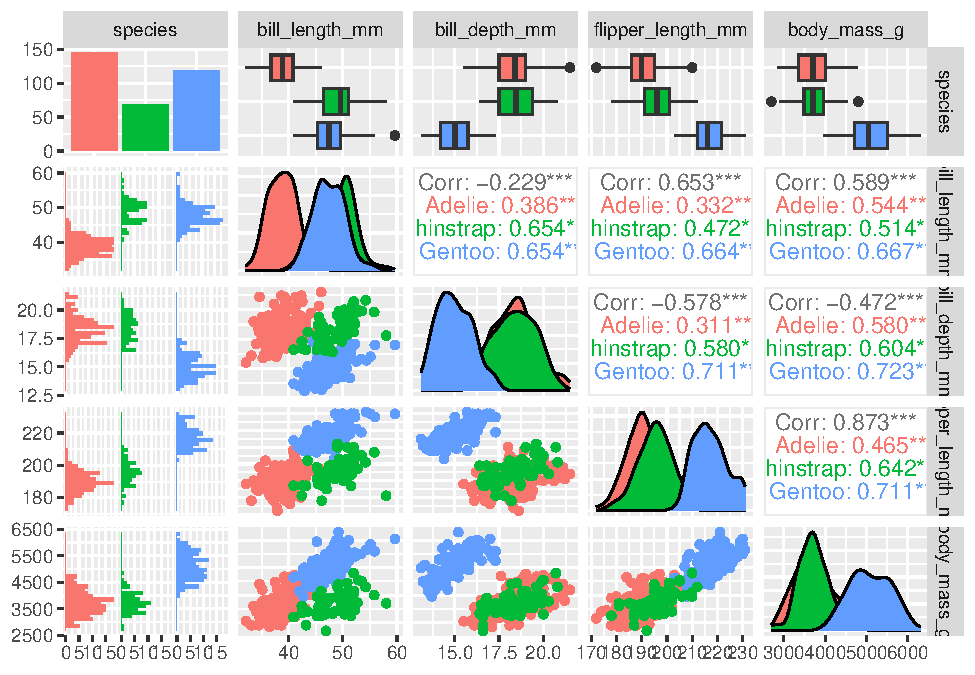
\includegraphics{EDA_files/figure-latex/unnamed-chunk-37-1.pdf}

\hypertarget{how-can-i-save-plots}{%
\subsubsection{How can I save plots?}\label{how-can-i-save-plots}}

There are many ways to save a ggplot:

\begin{itemize}
\item
  Go to the bottom right windows of RStudio. Plots \textgreater{} Export
  \textgreater{} Save as PDF,
\item
  Using the \texttt{ggsave("r-graphics.pdf",\ plot\_obj)} function from
  the \texttt{ggplot2} package, where \texttt{r-graphics.pdf} is the
  file name to create on disk and \texttt{plot\_obj} is the plot to
  save.
\item
  Open a graphic device, i.e., \texttt{pdf("r-graphics.pdf")}, create
  and print a plot, and finally close the graphic device using the
  function \texttt{dev.off()}.
\end{itemize}

\hypertarget{exercises}{%
\subsection{Exercises}\label{exercises}}

\hypertarget{exercise-6}{%
\subsubsection{Exercise 6}\label{exercise-6}}

Write a function named \texttt{kurtosis} to calculate the kurtosis
indices \(k_1\) and \(k_2\) given in the formulas:

\[
k_1 = \frac{\sum_{i=1}^N (Y_i - \bar{Y})^4 / N}{s^4}
\]

\[
k_2 = \frac{\sum_{i=1}^N (Y_i - \bar{Y})^4 / N}{s^4} - 3
\]

Write a function named \texttt{skewness} is a similar way.

\hypertarget{exercise-7}{%
\subsubsection{Exercise 7}\label{exercise-7}}

The data file \texttt{fondi.txt} contains the returns of 30 funds
categorized into two types labeled \texttt{A} and \texttt{B}. Analyze
the two variables separately. Specifically:

\begin{enumerate}
\def\labelenumi{\arabic{enumi}.}
\tightlist
\item
  Create a table with the minimum, \(Q_1\), mean, median, \(Q_3\),
  maximum, standard deviation, and interquartile range for both
  variables, rounded to two decimal places.
\item
  Plot the density and empirical cumulative distribution functions for
  each variable separately.
\item
  Compute skewness and kurtosis indices.
\item
  Compare the two variables using boxplots and empirical cumulative
  distribution functions after standardizing the data.
\end{enumerate}

Comment on the results.

\end{document}
